\chapter{Conception et Architecture du Système}

\section{Recueil et spécification des besoins}

La phase de recueil et de spécification des besoins constitue le fondement de toute démarche d'ingénierie logicielle rigoureuse. Elle permet d'établir un contrat clair entre les parties prenantes et l'équipe de développement, en formalisant les attentes fonctionnelles et les contraintes non fonctionnelles du système. Dans le cadre de Hostifer, cette phase revêt une importance particulière, car la plateforme doit répondre simultanément aux exigences d'une infrastructure multi-tenant à haute disponibilité, aux contraintes réglementaires algériennes, et aux attentes d'utilisabilité propres aux développeurs. Les besoins ont été recueillis par une analyse itérative combinant l'étude des solutions existantes (menée au chapitre précédent) et la modélisation des cas d'usage réels identifiés lors de la conception.

% ------------------------------------------------------------
\% ------------------------------------------------------------
\subsection{Identification des acteurs}
% ------------------------------------------------------------

Au sens de la norme UML~2.5, un acteur est un \textit{behaviored classifier} qui modélise le rôle joué par une entité externe au système, qu'il s'agisse d'un utilisateur humain, d'un système logiciel tiers ou d'un composant matériel, et qui interagit avec le sujet par échange de signaux et de données \cite{uml-spec}. L'acteur est, par définition, placé en dehors de la frontière du système ; il n'en fait pas partie mais en déclenche ou en consulte les comportements observables \cite{booch-uml}. L'identification rigoureuse des acteurs est une étape préalable à toute modélisation des cas d'utilisation, car elle délimite le périmètre du système et constitue le point de départ de l'élicitation des besoins \cite{sommerville-se}.

Pour Hostifer, l'analyse des diagrammes de séquence et des flux d'interaction a permis d'identifier deux catégories d'acteurs : les \textbf{acteurs humains}, qui initient des actions via une interface utilisateur, et les \textbf{acteurs systèmes}, qui interagissent avec la plateforme de manière automatisée, soit en tant que systèmes externes déclencheurs, soit en tant que composants d'infrastructure participant aux workflows internes. Le tableau~\ref{tab:acteurs} présente la synthèse complète des acteurs identifiés.

\subsubsection*{Acteurs humains}

\textbf{L'Utilisateur (Développeur)} est l'acteur principal de la plateforme. Il représente tout profil de développeur souhaitant déployer et opérer des applications web sans gérer directement l'infrastructure sous-jacente : ingénieur logiciel, freelance, membre d'une startup ou d'une PME. L'utilisateur interagit avec Hostifer exclusivement via le \textbf{frontend Next.js}, qui constitue le point d'entrée graphique de la plateforme. Ses actions couvrent l'ensemble du cycle de vie applicatif : authentification, création et configuration de projets, déclenchement de déploiements, consultation des journaux de build en temps réel, gestion des variables d'environnement, et activation du pipeline CI/CD automatique.

\textbf{L'Administrateur de la plateforme} est un acteur humain secondaire disposant de droits étendus sur l'ensemble du système. Il supervise la santé de l'infrastructure, gère les plans tarifaires et les quotas de ressources par tenant, et intervient en cas d'incident. L'administrateur interagit principalement avec les outils d'observabilité et d'orchestration (tableaux de bord Grafana, interface Argo Workflows UI) ainsi qu'avec les API d'administration exposées par le \textbf{backend NestJS}.

\subsubsection*{Acteurs systèmes externes}

\textbf{NextAuth.js} est la bibliothèque d'authentification intégrée au frontend Next.js. Elle gère les sessions utilisateur côté client, orchestre le flux OAuth~2.0 vers GitHub, et délègue l'émission et le renouvellement des jetons JWT au backend NestJS via des callbacks configurables. Bien qu'elle soit un composant interne au frontend, son rôle de médiateur entre l'utilisateur, le fournisseur OAuth et le backend en fait un participant structurant des diagrammes d'interaction.

\textbf{GitHub OAuth} est le fournisseur d'identité externe utilisé pour l'authentification déléguée. Lors d'une connexion via OAuth~2.0, GitHub valide l'identité de l'utilisateur et retourne un code d'autorisation que NextAuth.js échange contre un jeton d'accès. En complément, \textbf{GitHub} agit comme système déclencheur du pipeline CI/CD : à chaque événement \texttt{push} sur une branche configurée, il émet une requête HTTP vers l'endpoint webhook du backend NestJS, initiant automatiquement un nouveau déploiement sans intervention humaine.

\subsubsection*{Acteurs systèmes d'orchestration et d'infrastructure}

\textbf{Argo Workflows} est le moteur d'orchestration des pipelines de déploiement. Il reçoit les soumissions de \textit{WorkflowTemplates} depuis le backend NestJS via l'API REST Argo, puis exécute séquentiellement les trois étapes du pipeline : \textit{Build}, \textit{Provision} et \textit{DNS}. Argo Workflows interagit directement avec l'\textbf{API Kubernetes} pour créer et surveiller les ressources d'exécution de chaque étape.

\textbf{Le Builder Job (Go)} est le composant exécuté sous forme de Job Kubernetes lors de l'étape \textit{Build}. Ce binaire Go orchestre la chaîne de construction complète : clonage du dépôt Git, invocation de \textbf{Railpack CLI} pour la détection du framework et la génération du plan de build, connexion au daemon \textbf{Buildkitd} pour la construction de l'image OCI, et push de l'image résultante vers le \textbf{registre interne (Registry OCI)}.

\textbf{Helm} est le gestionnaire de packages Kubernetes utilisé lors de l'étape \textit{Provision}. Il déploie ou met à jour le chart Helm dédié à chaque tenant, créant l'ensemble des ressources Kubernetes nécessaires : \textit{Namespace}, \textit{Deployment}, \textit{Service}, \textit{NetworkPolicy}, \textit{ResourceQuota}, \textit{HorizontalPodAutoscaler} et \textit{ExternalSecret}.

\textbf{L'API Kubernetes} est le point d'entrée central de l'infrastructure d'exécution. Elle est sollicitée par Argo Workflows, par Helm et directement par le backend NestJS pour la création, la mise à jour et la suppression de l'ensemble des ressources Kubernetes associées aux tenants \cite{k8s-concepts}.

\textbf{Vault + ESO (External Secrets Operator)} constituent le sous-système de gestion des secrets. HashiCorp Vault stocke les variables d'environnement sensibles des tenants dans un moteur KV~v2 chiffré. L'External Secrets Operator synchronise ces secrets vers des ressources \textit{Kubernetes Secret} natives, qui sont ensuite injectées dans les pods applicatifs via \texttt{envFrom}, sans que les valeurs ne transitent jamais en clair.

\textbf{Traefik} est le contrôleur d'entrée (\textit{Ingress Controller}) du cluster. Il assure le routage du trafic HTTP/HTTPS entrant vers les services des tenants selon les règles d'IngressRoute définies par le chart Helm, et s'intègre avec \textbf{cert-manager} pour le provisionnement et le renouvellement automatiques des certificats TLS via Let's Encrypt.

\textbf{Promtail (DaemonSet) et Loki} forment le sous-système de collecte et d'indexation des journaux. Promtail, déployé en tant que DaemonSet sur chaque nœud du cluster, collecte les flux \texttt{stdout} des pods de construction et y attache des labels structurés (\texttt{build\_id}, \texttt{tenant\_id}, \texttt{log\_type}). Les journaux sont transmis à Loki pour indexation et persistance, depuis lesquels le backend NestJS les interroge via l'API \texttt{query\_range} pour les diffuser en temps réel à l'utilisateur via SSE (\textit{Server-Sent Events}).

\begin{table}[htbp]
\caption{Synthèse des acteurs du système Hostifer}
\label{tab:acteurs}
\centering
\renewcommand{\arraystretch}{1.3}
\begin{tabular}{|p{3.2cm}|p{2.2cm}|p{2.2cm}|p{5.5cm}|}
\hline
\textbf{Acteur} & \textbf{Type} & \textbf{Catégorie} & \textbf{Rôle principal} \\
\hline
Utilisateur & Humain & Principal & Déploie et opère ses applications via le frontend Next.js \\
\hline
Administrateur & Humain & Secondaire & Supervise la plateforme et l'infrastructure \\
\hline
NextAuth.js & Système interne & Secondaire & Gère les sessions et orchestre le flux OAuth côté frontend \\
\hline
GitHub OAuth & Système externe & Secondaire & Fournisseur d'identité OAuth~2.0 \\
\hline
GitHub (webhook) & Système externe & Déclencheur & Déclenche le CI/CD via événement \texttt{push} \\
\hline
Argo Workflows & Système interne & Orchestrateur & Exécute les pipelines Build / Provision / DNS \\
\hline
Builder Job (Go) & Système interne & Automatisé & Construit et pousse l'image OCI via Railpack et Buildkitd \\
\hline
Railpack CLI & Système interne & Automatisé & Détecte le framework et génère le plan de build \\
\hline
Buildkitd & Système interne & Automatisé & Construit l'image OCI à partir du plan Railpack \\
\hline
Registry (OCI) & Système interne & Automatisé & Stocke les images OCI des applications \\
\hline
Kubernetes API & Système interne & Infrastructure & Point d'entrée pour toutes les opérations sur les ressources cluster \\
\hline
Helm & Système interne & Infrastructure & Provisionne les ressources Kubernetes par tenant via chart \\
\hline
Vault + ESO & Système interne & Sécurité & Stocke et injecte les secrets applicatifs chiffrés \\
\hline
cert-manager & Système interne & Infrastructure & Émet et renouvelle les certificats TLS automatiquement \\
\hline
Traefik & Système interne & Infrastructure & Route le trafic entrant et assure la terminaison TLS \\
\hline
Loki & Système interne & Observabilité & Indexe et persiste les journaux des pods \\
\hline
Promtail (DaemonSet) & Système interne & Observabilité & Collecte les journaux des pods et les transmet à Loki \\
\hline
\end{tabular}
\end{table}
% ------------------------------------------------------------
\subsection{Besoins fonctionnels}
% ------------------------------------------------------------

Les besoins fonctionnels décrivent l'ensemble des services que le système doit fournir à ses utilisateurs ainsi que les comportements attendus en réponse à des entrées spécifiques \cite{sommerville-se}. Ils ont été structurés en sept domaines fonctionnels cohérents avec les grands cas d'utilisation de la plateforme, et priorisés selon la méthode MoSCoW (\textit{Must have}, \textit{Should have}, \textit{Could have}, \textit{Won't have}) \cite{moscow-ieee}, qui permet d'aligner les efforts de développement sur les fonctionnalités à plus fort impact métier.

\textbf{Authentification et gestion des comptes.} La plateforme doit permettre à tout utilisateur de s'inscrire et de s'authentifier, soit par une paire identifiant/mot de passe avec hachage sécurisé, soit par le protocole OAuth 2.0 délégué à GitHub. Le système doit émettre et renouveler des jetons d'accès JWT (\textit{JSON Web Token}) de manière transparente, avec un mécanisme de rotation des jetons de rafraîchissement afin de maintenir la sécurité des sessions longues.

\textbf{Gestion des projets.} Un développeur authentifié doit pouvoir créer un projet en fournissant l'URL d'un dépôt GitHub, configurer ses paramètres (région de déploiement, plan tarifaire associé), consulter la liste de ses projets avec leur statut en temps réel, et supprimer un projet avec déprovisionning complet des ressources Kubernetes associées.

\textbf{Déploiement d'applications.} La fonctionnalité centrale de la plateforme consiste à déployer automatiquement une application depuis un dépôt GitHub vers l'infrastructure Kubernetes. Ce processus doit couvrir la détection automatique du framework utilisé, la construction de l'image conteneur via Railpack et Buildkit, son stockage dans un registre interne, et son déploiement via un chart Helm dédié par tenant. L'utilisateur doit avoir accès à l'historique complet des déploiements et pouvoir effectuer un retour arrière vers une version stable antérieure.

\textbf{Journalisation en temps réel.} Pendant et après le processus de construction, l'utilisateur doit pouvoir consulter les journaux de build en continu, sans rechargement de page, via une connexion SSE (\textit{Server-Sent Events}). Les journaux doivent être indexés et persistés dans Loki afin d'être consultables a posteriori.

\textbf{Gestion des variables d'environnement.} La plateforme doit permettre la création, la mise à jour et la suppression de variables d'environnement associées à chaque projet. Les valeurs sensibles (secrets) doivent être stockées de manière chiffrée dans HashiCorp Vault et jamais exposées en clair dans l'interface ou dans les journaux.

\textbf{Intégration et livraison continues (CI/CD).} Le système doit permettre la configuration d'un pipeline CI/CD automatique, déclenché par un événement \texttt{push} GitHub via webhook. L'utilisateur doit pouvoir activer ou désactiver ce comportement par projet, et choisir la branche de déploiement cible.

\textbf{Administration de la plateforme.} L'administrateur doit disposer d'une interface permettant de visualiser l'ensemble des tenants actifs, leur consommation de ressources, et les workflows Argo Workflows en cours d'exécution. Il doit pouvoir intervenir sur les ressources Kubernetes directement depuis les outils d'observabilité intégrés.

Le tableau~\ref{tab:besoins-fonctionnels} synthétise l'ensemble des besoins fonctionnels avec leur identifiant, leur description, leur priorité MoSCoW et l'acteur concerné.

\begin{table}[htbp]
\caption{Tableau des besoins fonctionnels}
\label{tab:besoins-fonctionnels}
\centering
\renewcommand{\arraystretch}{1.3}
\begin{tabular}{|p{1.1cm}|p{5.5cm}|p{2cm}|p{3.5cm}|}
\hline
\textbf{ID} & \textbf{Description} & \textbf{Priorité} & \textbf{Acteur concerné} \\
\hline
BF-01 & S'inscrire avec email/mot de passe & Must have & Développeur \\
\hline
BF-02 & S'authentifier via OAuth GitHub & Must have & Développeur \\
\hline
BF-03 & Émettre et renouveler des jetons JWT & Must have & Système (NestJS) \\
\hline
BF-04 & Créer un projet depuis une URL GitHub & Must have & Développeur \\
\hline
BF-05 & Consulter la liste des projets et leurs statuts & Must have & Développeur \\
\hline
BF-06 & Déclencher manuellement un déploiement & Must have & Développeur \\
\hline
BF-07 & Détecter automatiquement le framework applicatif & Must have & Système (Builder Go) \\
\hline
BF-08 & Construire l'image conteneur via Buildkit/Railpack & Must have & Système (Argo Workflows) \\
\hline
BF-09 & Déployer l'application via chart Helm & Must have & Système (Argo Workflows) \\
\hline
BF-10 & Consulter les journaux de build en temps réel (SSE) & Must have & Développeur \\
\hline
BF-11 & Gérer les variables d'environnement (CRUD) & Must have & Développeur \\
\hline
BF-12 & Stocker les secrets dans HashiCorp Vault & Must have & Système (NestJS/ESO) \\
\hline
BF-13 & Configurer le déploiement automatique sur push GitHub & Should have & Développeur \\
\hline
BF-14 & Consulter l'historique des déploiements & Should have & Développeur \\
\hline
BF-15 & Effectuer un retour arrière vers une version précédente & Should have & Développeur \\
\hline
BF-16 & Supprimer un projet avec déprovisionning Kubernetes & Must have & Développeur \\
\hline
BF-17 & Gérer les membres d'une équipe projet & Should have & Développeur \\
\hline
BF-18 & Administrer les tenants et ressources (interface admin) & Must have & Administrateur \\
\hline
BF-19 & Visualiser les workflows Argo en cours & Should have & Administrateur \\
\hline
BF-20 & Configurer un domaine personnalisé & Could have & Développeur \\
\hline
\end{tabular}
\end{table}

% ------------------------------------------------------------
\subsection{Besoins non fonctionnels}
% ------------------------------------------------------------

Les besoins non fonctionnels définissent les contraintes de qualité auxquelles le système doit se conformer, indépendamment des fonctionnalités qu'il offre. Ils couvrent des attributs tels que la performance, la disponibilité, la sécurité et la scalabilité, et constituent souvent les critères les plus déterminants pour l'expérience utilisateur réelle et la viabilité opérationnelle de la plateforme \cite{sommerville-se}. Dans le contexte d'une plateforme PaaS multi-tenant comme Hostifer, ces exigences sont particulièrement critiques, car une dégradation dans l'un de ces domaines peut simultanément affecter l'ensemble des tenants hébergés sur l'infrastructure partagée.

\textbf{Performance.} Le temps de déploiement de bout en bout, mesuré depuis la soumission du workflow Argo jusqu'au passage de l'application à l'état \texttt{LIVE}, ne doit pas excéder cinq minutes pour les frameworks courants (Express, NestJS, Next.js, Flask) sur un dépôt de taille standard. La latence de streaming des journaux de build via SSE doit rester inférieure à deux secondes entre l'émission d'un message par le pod de construction et son affichage dans le navigateur de l'utilisateur.

\textbf{Disponibilité.} La plateforme cible un SLA (\textit{Service Level Agreement}) de disponibilité de 99,5\% pour les plans Standard, et de 99,9\% pour les plans Enterprise, ce qui correspond à une indisponibilité maximale tolérée respectivement de 43,8 heures et 8,76 heures par an. Ces objectifs imposent une architecture résiliente aux défaillances de composants individuels, notamment via la redondance des pods applicatifs et la gestion des interruptions planifiées.

\textbf{Sécurité.} L'isolation réseau entre tenants doit être garantie par des \textit{NetworkPolicies} Kubernetes bloquant tout trafic inter-namespace non autorisé \cite{multitenant-cloud}. Les secrets applicatifs ne doivent jamais transiter en clair : leur cycle de vie complet (création, stockage, injection dans les pods) est pris en charge par HashiCorp Vault et l'opérateur External Secrets. Les communications entre l'utilisateur et la plateforme doivent être intégralement chiffrées via TLS, avec émission et renouvellement automatiques des certificats assurés par cert-manager et Let's Encrypt. L'accès aux ressources Kubernetes est contrôlé par des politiques RBAC (\textit{Role-Based Access Control}) granulaires, limitant strictement les permissions de chaque composant.

\textbf{Scalabilité et autoscaling.} La plateforme doit supporter une montée en charge dynamique à trois niveaux distincts \cite{k8s-autoscaling}, correspondant aux trois couches de l'architecture Kubernetes.

Au niveau des pods, le \textit{Horizontal Pod Autoscaler} (HPA) ajuste automatiquement le nombre de réplicas d'un déploiement en fonction de métriques observées telles que l'utilisation CPU ou mémoire, ou de métriques applicatives personnalisées exposées via Prometheus Adapter \cite{k8s-hpa}. Le HPA est configuré avec des seuils de tolérance adaptés afin d'éviter les phénomènes d'oscillation (\textit{flapping}) dus à des variations métrique transitoires. En complément, le \textit{Vertical Pod Autoscaler} (VPA) opère sur la dimension verticale en ajustant les champs \texttt{requests} et \texttt{limits} des conteneurs sur la base de l'historique de consommation réelle \cite{kubecost-vpa}. En mode \texttt{recommendation}, il fournit des suggestions sans perturber les pods en cours d'exécution ; en mode \texttt{auto}, il peut procéder à l'éviction et au redémarrage des pods pour appliquer les nouvelles valeurs. Afin d'éviter tout conflit avec le HPA sur les mêmes métriques, le VPA est configuré pour opérer sur des métriques distinctes lorsque les deux mécanismes coexistent \cite{k8s-hpa-vpa-conflict}.

Au niveau du cluster, des \textit{node pools} classés par profil de ressources (small, medium, large) permettent d'affecter les workloads aux nœuds les mieux dimensionnés selon le plan tarifaire du tenant. Le \textit{Cluster Autoscaler} surveille en permanence l'état des pods en attente de scheduling (\textit{Pending}) et des nœuds sous-utilisés, ajoutant de nouveaux nœuds lorsque la demande dépasse la capacité disponible et en retirant lorsque des nœuds restent inactifs sur une période prolongée \cite{k8s-autoscaling}.

Les \textit{ResourceQuotas} et les \textit{LimitRanges} définis par namespace délimitent les bornes minimales et maximales de consommation de ressources par tenant. Ces contraintes coopèrent avec le HPA et le VPA en empêchant les recommandations d'autoscaling de dépasser les quotas alloués par plan, garantissant ainsi la préservation de l'isolation multi-tenant même en période de forte charge \cite{microsoft-tenancy}.

\textbf{Maintenabilité.} L'architecture modulaire du backend NestJS (un module par domaine fonctionnel), l'utilisation de charts Helm paramétrables pour le provisionnement des tenants, et la séparation stricte des composants (frontend, backend, builder, infrastructure) doivent permettre la mise à jour et le débogage indépendants de chaque couche du système sans affecter les tenants en production.

Le tableau~\ref{tab:besoins-non-fonctionnels} récapitule l'ensemble des besoins non fonctionnels avec leurs critères de satisfaction mesurables.

\small
\setlength{\LTleft}{0pt}
\setlength{\LTright}{0pt}
\renewcommand{\arraystretch}{1.15}
\begin{longtable}{|p{1.1cm}|p{2.3cm}|>{\raggedright\arraybackslash}p{4.8cm}|>{\raggedright\arraybackslash}p{4cm}|}
\caption{Tableau des besoins non fonctionnels}\label{tab:besoins-non-fonctionnels}\\
\hline
\textbf{ID} & \textbf{Catégorie} & \textbf{Description} & \textbf{Critère de satisfaction} \\
\hline
\endfirsthead

\hline
\textbf{ID} & \textbf{Catégorie} & \textbf{Description} & \textbf{Critère de satisfaction} \\
\hline
\endhead

BNF-01 & Performance & Temps de déploiement de bout en bout & $\leq$ 5 min pour frameworks standard \\
\hline
BNF-02 & Performance & Latence de streaming des logs SSE & $\leq$ 2 s entre émission pod et affichage navigateur \\
\hline
BNF-03 & Disponibilité & SLA plan Standard & $\geq$ 99,5\% (43,8 h d'indisponibilité/an max.) \\
\hline
BNF-04 & Disponibilité & SLA plan Enterprise & $\geq$ 99,9\% (8,76 h d'indisponibilité/an max.) \\
\hline
BNF-05 & Sécurité & Isolation réseau inter-tenant & Zéro trafic inter-namespace validé par NetworkPolicy \\
\hline
BNF-06 & Sécurité & Chiffrement des secrets & Secrets stockés dans Vault KV v2, jamais en clair \\
\hline
BNF-07 & Sécurité & Chiffrement des communications & TLS obligatoire, certificats émis par cert-manager \\
\hline
BNF-08 & Sécurité & Contrôle d'accès & RBAC Kubernetes par namespace et par composant \\
\hline
BNF-09 & Scalabilité & Autoscaling horizontal des pods (HPA) & Augmentation du nombre de réplicas en $\leq$ 30 s sous charge CPU $>$ 70\% \\
\hline
BNF-10 & Scalabilité & Autoscaling vertical des pods (VPA) & Recommandations \texttt{requests}/\texttt{limits} appliquées sans interruption en mode \texttt{recommendation} \\
\hline
BNF-11 & Scalabilité & Autoscaling du cluster (Cluster Autoscaler) & Ajout/suppression automatique de nœuds en $\leq$ 3 min selon utilisation des ressources \\
\hline
BNF-12 & Scalabilité & Isolation des quotas multi-tenant & ResourceQuota empêche tout dépassement du plan tarifaire, même en cas de scaling \\
\hline
BNF-13 & Maintenabilité & Modularité du backend & Mise à jour d'un module NestJS sans impact sur les autres \\
\hline
BNF-14 & Maintenabilité & Paramétrabilité de l'infrastructure & Provisionnement complet d'un nouveau tenant via chart Helm sans modification manuelle \\
\hline
\end{longtable}
\normalsize

\section{Modélisation UML des cas d'utilisation}
% ------------------------------------------------------------
\subsection{Cas d'utilisation détaillés}
% ------------------------------------------------------------

Les cas d'utilisation suivants sont décrits selon le format textuel standard préconisé pour les mémoires de fin d'études en informatique. Chaque fiche précise le nom du cas d'utilisation, l'acteur principal, les préconditions requises, le scénario nominal (flux de succès), les scénarios alternatifs et d'exception, ainsi que les postconditions observables à l'issue de l'interaction.

% Macro de mise en forme commune pour toutes les fiches CU
\newcommand{\cucell}[1]{\textbf{#1}}

% ── CU01 ────────────────────────────────────────────────────
% \begin{table}[htbp]
% \caption{CU01 — S'authentifier}
% \label{tab:cu01}
% \centering
% \renewcommand{\arraystretch}{1.4}
% \begin{tabular}{|p{3.5cm}|p{10cm}|}
% \hline
% \cucell{Identifiant} & CU01 \\
% \hline
% \cucell{Nom} & S'authentifier \\
% \hline
% \cucell{Acteur principal} & Utilisateur \\
% \hline
% \cucell{Acteurs secondaires} & NextAuth.js, NestJS API, GitHub OAuth, PostgreSQL \\
% \hline
% \cucell{Préconditions} &
% \begin{minipage}[t]{10cm}
% \begin{itemize}[nosep, left=0pt]
%   \item L'utilisateur possède un compte enregistré sur la plateforme, ou un compte GitHub valide.
%   \item Le service NestJS API est disponible.
%   \item La connexion au fournisseur OAuth GitHub est opérationnelle.
% \end{itemize}
% \end{minipage} \\
% \hline
% \cucell{Scénario nominal} &
% \begin{minipage}[t]{10cm}
% \begin{enumerate}[nosep, left=0pt]
%   \item L'utilisateur accède à la page de connexion du frontend Next.js.
%   \item L'utilisateur saisit son adresse email et son mot de passe, puis soumet le formulaire.
%   \item NextAuth.js transmet les identifiants au backend NestJS via l'endpoint \texttt{POST /auth/login}.
%   \item NestJS vérifie les identifiants contre la base de données PostgreSQL et valide le hachage du mot de passe.
%   \item NestJS émet une paire de jetons : un jeton d'accès JWT (courte durée de vie) et un jeton de rafraîchissement (longue durée de vie).
%   \item NextAuth.js stocke les jetons dans la session côté client et redirige l'utilisateur vers son tableau de bord.
% \end{enumerate}
% \end{minipage} \\
% \hline
% \cucell{Scénarios alternatifs} &
% \begin{minipage}[t]{10cm}
% \textbf{A1 — Authentification via OAuth GitHub :}
% \begin{enumerate}[nosep, left=0pt]
%   \item L'utilisateur clique sur « Continuer avec GitHub ».
%   \item NextAuth.js redirige le navigateur vers le serveur d'autorisation GitHub OAuth.
%   \item L'utilisateur autorise l'accès à son compte GitHub.
%   \item GitHub retourne un code d'autorisation ; NextAuth.js l'échange contre un token d'accès GitHub.
%   \item NestJS reçoit le profil GitHub, crée ou met à jour le compte utilisateur dans PostgreSQL, et émet les jetons JWT.
%   \item L'utilisateur est redirigé vers son tableau de bord.
% \end{enumerate}
% \vspace{4pt}
% \textbf{A2 — Jeton d'accès expiré :}
% \begin{enumerate}[nosep, left=0pt]
%   \item Le callback \texttt{jwt} de NextAuth.js détecte que le jeton d'accès est expiré.
%   \item NextAuth.js appelle automatiquement \texttt{POST /auth/refresh} avec le jeton de rafraîchissement.
%   \item NestJS valide le jeton de rafraîchissement, révoque l'ancien et émet une nouvelle paire de jetons.
%   \item La session est mise à jour de manière transparente, sans interruption pour l'utilisateur.
% \end{enumerate}
% \end{minipage} \\
% \hline
% \cucell{Scénarios d'exception} &
% \begin{minipage}[t]{10cm}
% \textbf{E1 — Identifiants incorrects :} NestJS retourne une erreur \texttt{401 Unauthorized} ; NextAuth.js affiche un message d'erreur à l'utilisateur. \\[4pt]
% \textbf{E2 — Jeton de rafraîchissement expiré ou révoqué :} NextAuth.js invalide la session et redirige l'utilisateur vers la page de connexion. \\[4pt]
% \textbf{E3 — Service NestJS indisponible :} NextAuth.js retourne une erreur de connexion ; l'utilisateur est invité à réessayer ultérieurement.
% \end{minipage} \\
% \hline
% \cucell{Postconditions} &
% \begin{minipage}[t]{10cm}
% \begin{itemize}[nosep, left=0pt]
%   \item L'utilisateur dispose d'une session active avec un jeton d'accès JWT valide.
%   \item L'utilisateur est redirigé vers son tableau de bord personnel.
% \end{itemize}
% \end{minipage} \\
% \hline
% \end{tabular}
% \end{table}

% % ── CU02 ────────────────────────────────────────────────────
% \begin{table}[htbp]
% \caption{CU02 — Créer un projet depuis une URL GitHub}
% \label{tab:cu02}
% \centering
% \renewcommand{\arraystretch}{1.4}
% \begin{tabular}{|p{3.5cm}|p{10cm}|}
% \hline
% \cucell{Identifiant} & CU02 \\
% \hline
% \cucell{Nom} & Créer un projet depuis une URL GitHub \\
% \hline
% \cucell{Acteur principal} & Utilisateur \\
% \hline
% \cucell{Acteurs secondaires} & NestJS API, GitHub OAuth, PostgreSQL \\
% \hline
% \cucell{Préconditions} &
% \begin{minipage}[t]{10cm}
% \begin{itemize}[nosep, left=0pt]
%   \item L'utilisateur est authentifié (CU01 accompli).
%   \item L'utilisateur a installé l'application GitHub de la plateforme sur son compte ou son organisation GitHub.
%   \item Le dépôt GitHub cible est accessible par l'installation GitHub de la plateforme.
% \end{itemize}
% \end{minipage} \\
% \hline
% \cucell{Scénario nominal} &
% \begin{minipage}[t]{10cm}
% \begin{enumerate}[nosep, left=0pt]
%   \item L'utilisateur accède à la page de création de projet et saisit l'URL du dépôt GitHub.
%   \item Le frontend transmet l'URL et les paramètres choisis (nom du projet, plan tarifaire) au backend via \texttt{POST /projects}.
%   \item NestJS vérifie que l'installation GitHub associée à l'utilisateur a bien accès au dépôt spécifié.
%   \item NestJS crée un enregistrement \texttt{Project} dans PostgreSQL avec le statut \texttt{CREATED}.
%   \item NestJS enregistre un webhook sur le dépôt GitHub via l'API GitHub pour les événements \texttt{push}.
%   \item Le frontend redirige l'utilisateur vers la page de détail du projet nouvellement créé.
% \end{enumerate}
% \end{minipage} \\
% \hline
% \cucell{Scénarios alternatifs} &
% \begin{minipage}[t]{10cm}
% \textbf{A1 — L'installation GitHub n'est pas encore configurée :}
% \begin{enumerate}[nosep, left=0pt]
%   \item Le frontend détecte l'absence d'installation GitHub active.
%   \item L'utilisateur est redirigé vers la page d'installation de l'application GitHub de la plateforme.
%   \item Après installation, l'utilisateur reprend le flux de création à l'étape 1.
% \end{enumerate}
% \end{minipage} \\
% \hline
% \cucell{Scénarios d'exception} &
% \begin{minipage}[t]{10cm}
% \textbf{E1 — Dépôt inaccessible ou URL invalide :} NestJS retourne \texttt{404 Not Found} ; le frontend affiche un message indiquant que le dépôt est introuvable ou non autorisé. \\[4pt]
% \textbf{E2 — Nom de projet déjà utilisé :} NestJS retourne \texttt{409 Conflict} ; l'utilisateur est invité à choisir un nom différent.
% \end{minipage} \\
% \hline
% \cucell{Postconditions} &
% \begin{minipage}[t]{10cm}
% \begin{itemize}[nosep, left=0pt]
%   \item Un enregistrement \texttt{Project} est créé en base de données avec le statut \texttt{CREATED}.
%   \item Un webhook GitHub est enregistré sur le dépôt pour les événements \texttt{push}.
%   \item Le projet est visible dans le tableau de bord de l'utilisateur.
% \end{itemize}
% \end{minipage} \\
% \hline
% \end{tabular}
% \end{table}

% % ── CU03 ────────────────────────────────────────────────────
% \begin{table}[htbp]
% \caption{CU03 — Configurer et déclencher un déploiement}
% \label{tab:cu03}
% \centering
% \renewcommand{\arraystretch}{1.4}
% \begin{tabular}{|p{3.5cm}|p{10cm}|}
% \hline
% \cucell{Identifiant} & CU03 \\
% \hline
% \cucell{Nom} & Configurer et déclencher un déploiement \\
% \hline
% \cucell{Acteur principal} & Utilisateur \\
% \hline
% \cucell{Acteurs secondaires} & NestJS API, Argo Workflows, Builder Job (Go), Railpack CLI, Buildkitd, Registry OCI, Helm, Kubernetes API, PostgreSQL \\
% \hline
% \cucell{Préconditions} &
% \begin{minipage}[t]{10cm}
% \begin{itemize}[nosep, left=0pt]
%   \item L'utilisateur est authentifié (CU01 accompli).
%   \item Un projet a été créé (CU02 accompli).
%   \item Le dépôt GitHub associé au projet est non vide et contient un code source valide.
% \end{itemize}
% \end{minipage} \\
% \hline
% \cucell{Scénario nominal} &
% \begin{minipage}[t]{10cm}
% \begin{enumerate}[nosep, left=0pt]
%   \item L'utilisateur accède à la page du projet et clique sur « Déployer ».
%   \item Le frontend soumet la requête de déploiement au backend via \texttt{POST /deployments}.
%   \item NestJS crée un enregistrement \texttt{Deployment} en base avec le statut \texttt{QUEUED} et soumet un \textit{WorkflowTemplate} à Argo Workflows via son API REST.
%   \item \textbf{Étape Build :} Argo Workflows crée un Builder Job (Go) qui clone le dépôt, invoque Railpack CLI pour détecter le framework et générer le plan de build, puis construit l'image OCI via Buildkitd et la pousse vers le registre interne. Le statut passe à \texttt{BUILDING}.
%   \item \textbf{Étape Provision :} Argo Workflows invoque Helm pour déployer ou mettre à jour le chart Helm du tenant sur le cluster Kubernetes. Le statut passe à \texttt{PROVISIONING}.
%   \item \textbf{Étape DNS :} Argo Workflows configure les règles d'IngressRoute Traefik et déclenche l'émission du certificat TLS via cert-manager. Le statut passe à \texttt{CONFIGURING\_DNS}.
%   \item NestJS met à jour le statut du déploiement à \texttt{LIVE} et enregistre l'URL publique de l'application.
%   \item Le frontend affiche la confirmation du déploiement avec l'URL live de l'application.
% \end{enumerate}
% \end{minipage} \\
% \hline
% \cucell{Scénarios alternatifs} &
% \begin{minipage}[t]{10cm}
% \textbf{A1 — Redéploiement d'un projet existant :}
% \begin{enumerate}[nosep, left=0pt]
%   \item Si un déploiement actif existe déjà, Helm effectue une mise à jour (\texttt{helm upgrade}) plutôt qu'une installation initiale.
%   \item L'ancien pod reste actif jusqu'à ce que le nouveau soit en état \texttt{Running}, assurant une continuité de service.
% \end{enumerate}
% \end{minipage} \\
% \hline
% \cucell{Scénarios d'exception} &
% \begin{minipage}[t]{10cm}
% \textbf{E1 — Échec de l'étape Build :} Le Builder Job retourne une erreur (dépôt invalide, framework non reconnu, erreur de compilation) ; le statut passe à \texttt{FAILED} et les journaux d'erreur sont disponibles via SSE. \\[4pt]
% \textbf{E2 — Échec de l'étape Provision :} Helm retourne une erreur (quota dépassé, ressources insuffisantes) ; le statut passe à \texttt{FAILED}. \\[4pt]
% \textbf{E3 — Timeout du workflow :} Argo Workflows annule le workflow après dépassement du délai maximal ; le statut passe à \texttt{CANCELLED}.
% \end{minipage} \\
% \hline
% \cucell{Postconditions} &
% \begin{minipage}[t]{10cm}
% \begin{itemize}[nosep, left=0pt]
%   \item En cas de succès : l'application est accessible à son URL publique ; le statut du déploiement est \texttt{LIVE}.
%   \item En cas d'échec : le statut est \texttt{FAILED} ou \texttt{CANCELLED} ; l'état précédent de l'application (si existant) est préservé.
%   \item L'historique du déploiement est conservé en base de données avec les métadonnées de chaque étape.
% \end{itemize}
% \end{minipage} \\
% \hline
% \end{tabular}
% \end{table}

% % ── CU04 ────────────────────────────────────────────────────
% \begin{table}[htbp]
% \caption{CU04 — Consulter les journaux de build en temps réel}
% \label{tab:cu04}
% \centering
% \renewcommand{\arraystretch}{1.4}
% \begin{tabular}{|p{3.5cm}|p{10cm}|}
% \hline
% \cucell{Identifiant} & CU04 \\
% \hline
% \cucell{Nom} & Consulter les journaux de build en temps réel \\
% \hline
% \cucell{Acteur principal} & Utilisateur \\
% \hline
% \cucell{Acteurs secondaires} & NestJS API, Loki, Promtail (DaemonSet) \\
% \hline
% \cucell{Préconditions} &
% \begin{minipage}[t]{10cm}
% \begin{itemize}[nosep, left=0pt]
%   \item L'utilisateur est authentifié (CU01 accompli).
%   \item Un déploiement est en cours ou a été exécuté pour le projet concerné (CU03 déclenché).
%   \item Promtail est déployé en tant que DaemonSet sur les nœuds du cluster et collecte les flux \texttt{stdout} des pods de construction.
% \end{itemize}
% \end{minipage} \\
% \hline
% \cucell{Scénario nominal} &
% \begin{minipage}[t]{10cm}
% \begin{enumerate}[nosep, left=0pt]
%   \item L'utilisateur accède à la page de détail du déploiement (ou à l'assistant de déploiement à l'étape Build).
%   \item Le frontend ouvre une connexion SSE (\textit{Server-Sent Events}) vers l'endpoint \texttt{GET /deployments/:id/logs} du backend NestJS.
%   \item NestJS interroge l'API Loki (\texttt{query\_range}) toutes les deux secondes, filtrant les entrées par \texttt{build\_id} et \texttt{container="main"}.
%   \item Loki retourne les nouvelles lignes de journaux collectées par Promtail depuis le pod Builder Job.
%   \item NestJS diffuse chaque lot de lignes au frontend via le flux SSE.
%   \item Le frontend affiche les lignes dans l'interface de journaux en temps réel, en défilant automatiquement vers le bas.
%   \item Lorsque le déploiement atteint un état terminal (\texttt{LIVE}, \texttt{FAILED} ou \texttt{CANCELLED}), NestJS envoie un événement de fermeture et la connexion SSE est clôturée.
% \end{enumerate}
% \end{minipage} \\
% \hline
% \cucell{Scénarios alternatifs} &
% \begin{minipage}[t]{10cm}
% \textbf{A1 — Consultation des journaux d'un déploiement passé :}
% \begin{enumerate}[nosep, left=0pt]
%   \item L'utilisateur accède à l'historique des déploiements et sélectionne un déploiement terminé.
%   \item NestJS interroge Loki avec la plage temporelle correspondant à ce déploiement.
%   \item Les journaux sont retournés en une seule réponse (sans flux SSE continu) et affichés dans l'interface.
% \end{enumerate}
% \end{minipage} \\
% \hline
% \cucell{Scénarios d'exception} &
% \begin{minipage}[t]{10cm}
% \textbf{E1 — Loki indisponible :} NestJS retourne une erreur ; le frontend affiche un message indiquant que les journaux sont temporairement inaccessibles. \\[4pt]
% \textbf{E2 — Interruption réseau :} Le navigateur perd la connexion SSE ; le frontend tente une reconnexion automatique après un délai configurable.
% \end{minipage} \\
% \hline
% \cucell{Postconditions} &
% \begin{minipage}[t]{10cm}
% \begin{itemize}[nosep, left=0pt]
%   \item L'utilisateur a consulté les journaux de construction de son application.
%   \item Les journaux restent persistés dans Loki et consultables ultérieurement.
% \end{itemize}
% \end{minipage} \\
% \hline
% \end{tabular}
% \end{table}

% % ── CU05 ────────────────────────────────────────────────────
% \begin{table}[htbp]
% \caption{CU05 — Gérer les variables d'environnement}
% \label{tab:cu05}
% \centering
% \renewcommand{\arraystretch}{1.4}
% \begin{tabular}{|p{3.5cm}|p{10cm}|}
% \hline
% \cucell{Identifiant} & CU05 \\
% \hline
% \cucell{Nom} & Gérer les variables d'environnement \\
% \hline
% \cucell{Acteur principal} & Utilisateur \\
% \hline
% \cucell{Acteurs secondaires} & NestJS API, Vault + ESO, Kubernetes API, PostgreSQL \\
% \hline
% \cucell{Préconditions} &
% \begin{minipage}[t]{10cm}
% \begin{itemize}[nosep, left=0pt]
%   \item L'utilisateur est authentifié (CU01 accompli).
%   \item Un projet existe et l'utilisateur en est propriétaire ou membre autorisé (CU02 accompli).
%   \item HashiCorp Vault est disponible et le moteur KV~v2 du tenant est initialisé.
% \end{itemize}
% \end{minipage} \\
% \hline
% \cucell{Scénario nominal} &
% \begin{minipage}[t]{10cm}
% \begin{enumerate}[nosep, left=0pt]
%   \item L'utilisateur accède à l'onglet « Variables d'environnement » de la page du projet.
%   \item Le frontend affiche la liste des variables existantes avec leurs clés ; les valeurs sensibles sont masquées.
%   \item L'utilisateur ajoute, modifie ou supprime une ou plusieurs variables, puis valide.
%   \item Le frontend soumet les modifications au backend via \texttt{PUT /projects/:id/env-vars}.
%   \item NestJS écrit les nouvelles valeurs dans le chemin KV~v2 correspondant au tenant dans HashiCorp Vault, en s'authentifiant via la méthode Kubernetes Auth.
%   \item NestJS met à jour les métadonnées des variables (clés, types) dans PostgreSQL.
%   \item L'External Secrets Operator détecte la mise à jour du secret Vault et synchronise la ressource \textit{Kubernetes Secret} du namespace du tenant.
%   \item Les nouvelles variables sont disponibles dans les pods applicatifs lors du prochain redémarrage ou déploiement.
% \end{enumerate}
% \end{minipage} \\
% \hline
% \cucell{Scénarios alternatifs} &
% \begin{minipage}[t]{10cm}
% \textbf{A1 — Révélation temporaire d'une valeur secrète :}
% \begin{enumerate}[nosep, left=0pt]
%   \item L'utilisateur clique sur l'icône de démasquage d'une variable.
%   \item Le frontend appelle \texttt{GET /projects/:id/env-vars/:key/reveal}.
%   \item NestJS récupère la valeur depuis Vault et la retourne de manière chiffrée sur le canal HTTPS.
%   \item La valeur est affichée temporairement dans l'interface puis rémasquée automatiquement.
% \end{enumerate}
% \end{minipage} \\
% \hline
% \cucell{Scénarios d'exception} &
% \begin{minipage}[t]{10cm}
% \textbf{E1 — Vault indisponible :} NestJS retourne \texttt{503 Service Unavailable} ; les variables ne sont pas modifiées. \\[4pt]
% \textbf{E2 — Nom de variable invalide :} NestJS retourne \texttt{400 Bad Request} si la clé contient des caractères non autorisés.
% \end{minipage} \\
% \hline
% \cucell{Postconditions} &
% \begin{minipage}[t]{10cm}
% \begin{itemize}[nosep, left=0pt]
%   \item Les variables d'environnement sont mises à jour dans Vault KV~v2.
%   \item La ressource \textit{Kubernetes Secret} du tenant est synchronisée par ESO.
%   \item Aucune valeur sensible n'a transité en clair.
% \end{itemize}
% \end{minipage} \\
% \hline
% \end{tabular}
% \end{table}

% % ── CU06 ────────────────────────────────────────────────────
% \begin{table}[htbp]
% \caption{CU06 — Configurer le CI/CD (auto-déploiement sur push)}
% \label{tab:cu06}
% \centering
% \renewcommand{\arraystretch}{1.4}
% \begin{tabular}{|p{3.5cm}|p{10cm}|}
% \hline
% \cucell{Identifiant} & CU06 \\
% \hline
% \cucell{Nom} & Configurer le CI/CD (auto-déploiement sur push) \\
% \hline
% \cucell{Acteur principal} & Utilisateur \\
% \hline
% \cucell{Acteurs secondaires} & NestJS API, GitHub (webhook), Argo Workflows, PostgreSQL \\
% \hline
% \cucell{Préconditions} &
% \begin{minipage}[t]{10cm}
% \begin{itemize}[nosep, left=0pt]
%   \item L'utilisateur est authentifié (CU01 accompli).
%   \item Un projet a été créé et un premier déploiement a été effectué avec succès (CU02 et CU03 accomplis).
%   \item Un webhook GitHub est enregistré sur le dépôt (enregistré lors de CU02).
% \end{itemize}
% \end{minipage} \\
% \hline
% \cucell{Scénario nominal} &
% \begin{minipage}[t]{10cm}
% \begin{enumerate}[nosep, left=0pt]
%   \item L'utilisateur accède aux paramètres du projet et active l'option « Déploiement automatique ».
%   \item L'utilisateur sélectionne la branche de production à surveiller (ex. \texttt{main}).
%   \item Le frontend soumet la configuration au backend via \texttt{PATCH /projects/:id/settings}.
%   \item NestJS enregistre la configuration CI/CD en base de données (\texttt{auto\_deploy: true}, \texttt{branch: main}).
%   \item Lors d'un \texttt{push} ultérieur sur la branche configurée, GitHub émet une requête \texttt{POST} vers l'endpoint webhook \texttt{/webhooks/github}.
%   \item NestJS vérifie la signature HMAC du webhook, identifie le projet concerné, et déclenche automatiquement un nouveau déploiement (flux identique à CU03 à partir de l'étape 3).
% \end{enumerate}
% \end{minipage} \\
% \hline
% \cucell{Scénarios alternatifs} &
% \begin{minipage}[t]{10cm}
% \textbf{A1 — Désactivation du CI/CD :}
% \begin{enumerate}[nosep, left=0pt]
%   \item L'utilisateur désactive l'option « Déploiement automatique » dans les paramètres.
%   \item NestJS met à jour \texttt{auto\_deploy: false} en base.
%   \item Les événements webhook GitHub ultérieurs sont reçus mais ignorés pour ce projet.
% \end{enumerate}
% \end{minipage} \\
% \hline
% \cucell{Scénarios d'exception} &
% \begin{minipage}[t]{10cm}
% \textbf{E1 — Signature HMAC invalide :} NestJS rejette la requête webhook avec \texttt{401 Unauthorized} ; aucun déploiement n'est déclenché. \\[4pt]
% \textbf{E2 — Déploiement déjà en cours :} NestJS détecte un déploiement actif pour le projet ; le nouveau déclenchement est mis en file d'attente ou ignoré selon la politique configurée.
% \end{minipage} \\
% \hline
% \cucell{Postconditions} &
% \begin{minipage}[t]{10cm}
% \begin{itemize}[nosep, left=0pt]
%   \item La configuration CI/CD est persistée en base de données.
%   \item Tout \texttt{push} sur la branche configurée déclenche automatiquement un déploiement.
% \end{itemize}
% \end{minipage} \\
% \hline
% \end{tabular}
% \end{table}

% % ── CU07 ────────────────────────────────────────────────────
% \begin{table}[htbp]
% \caption{CU07 — Gérer les membres d'une équipe}
% \label{tab:cu07}
% \centering
% \renewcommand{\arraystretch}{1.4}
% \begin{tabular}{|p{3.5cm}|p{10cm}|}
% \hline
% \cucell{Identifiant} & CU07 \\
% \hline
% \cucell{Nom} & Gérer les membres d'une équipe \\
% \hline
% \cucell{Acteur principal} & Utilisateur (propriétaire du projet) \\
% \hline
% \cucell{Acteurs secondaires} & NestJS API, PostgreSQL \\
% \hline
% \cucell{Préconditions} &
% \begin{minipage}[t]{10cm}
% \begin{itemize}[nosep, left=0pt]
%   \item L'utilisateur est authentifié et est propriétaire du projet (CU01 et CU02 accomplis).
%   \item Le membre à inviter possède un compte enregistré sur la plateforme.
% \end{itemize}
% \end{minipage} \\
% \hline
% \cucell{Scénario nominal} &
% \begin{minipage}[t]{10cm}
% \begin{enumerate}[nosep, left=0pt]
%   \item L'utilisateur accède à l'onglet « Équipe » de la page du projet.
%   \item L'utilisateur saisit l'adresse email du membre à inviter et sélectionne son rôle (\textit{Viewer} ou \textit{Editor}).
%   \item Le frontend soumet l'invitation au backend via \texttt{POST /projects/:id/members}.
%   \item NestJS vérifie que l'email correspond à un compte existant, crée l'association dans PostgreSQL avec le rôle choisi.
%   \item Le membre invité peut désormais accéder au projet avec les droits correspondant à son rôle.
% \end{enumerate}
% \end{minipage} \\
% \hline
% \cucell{Scénarios alternatifs} &
% \begin{minipage}[t]{10cm}
% \textbf{A1 — Suppression d'un membre :}
% \begin{enumerate}[nosep, left=0pt]
%   \item Le propriétaire sélectionne un membre et clique sur « Retirer ».
%   \item NestJS supprime l'association du membre avec le projet en base de données.
%   \item Le membre ne peut plus accéder au projet.
% \end{enumerate}
% \end{minipage} \\
% \hline
% \cucell{Scénarios d'exception} &
% \begin{minipage}[t]{10cm}
% \textbf{E1 — Email non enregistré :} NestJS retourne \texttt{404 Not Found} ; l'utilisateur est informé que ce compte n'existe pas sur la plateforme. \\[4pt]
% \textbf{E2 — Membre déjà présent :} NestJS retourne \texttt{409 Conflict}.
% \end{minipage} \\
% \hline
% \cucell{Postconditions} &
% \begin{minipage}[t]{10cm}
% \begin{itemize}[nosep, left=0pt]
%   \item L'association membre-projet est persistée en base de données avec le rôle défini.
%   \item Le nouveau membre a accès au projet selon ses droits.
% \end{itemize}
% \end{minipage} \\
% \hline
% \end{tabular}
% \end{table}

% % ── CU08 ────────────────────────────────────────────────────
% \begin{table}[htbp]
% \caption{CU08 — Supprimer un projet (déprovisionning)}
% \label{tab:cu08}
% \centering
% \renewcommand{\arraystretch}{1.4}
% \begin{tabular}{|p{3.5cm}|p{10cm}|}
% \hline
% \cucell{Identifiant} & CU08 \\
% \hline
% \cucell{Nom} & Supprimer un projet (déprovisionning) \\
% \hline
% \cucell{Acteur principal} & Utilisateur (propriétaire du projet) \\
% \hline
% \cucell{Acteurs secondaires} & NestJS API, Kubernetes API, Helm, Vault + ESO, GitHub, PostgreSQL \\
% \hline
% \cucell{Préconditions} &
% \begin{minipage}[t]{10cm}
% \begin{itemize}[nosep, left=0pt]
%   \item L'utilisateur est authentifié et est propriétaire du projet (CU01 et CU02 accomplis).
%   \item Aucun déploiement n'est en cours pour ce projet.
% \end{itemize}
% \end{minipage} \\
% \hline
% \cucell{Scénario nominal} &
% \begin{minipage}[t]{10cm}
% \begin{enumerate}[nosep, left=0pt]
%   \item L'utilisateur accède aux paramètres du projet et clique sur « Supprimer le projet ».
%   \item Le frontend affiche une boîte de dialogue de confirmation demandant la saisie du nom du projet.
%   \item L'utilisateur confirme en saisissant le nom exact du projet.
%   \item Le frontend envoie la requête \texttt{DELETE /projects/:id} au backend NestJS.
%   \item NestJS supprime la release Helm du tenant via \texttt{helm uninstall}, ce qui entraîne la suppression de l'ensemble des ressources Kubernetes du namespace (Deployment, Service, IngressRoute, HPA, ExternalSecret).
%   \item NestJS supprime le namespace Kubernetes du tenant via l'API Kubernetes, ce qui entraîne la suppression de toutes les ressources restantes (NetworkPolicy, ResourceQuota, Secrets).
%   \item NestJS supprime le chemin KV~v2 correspondant au tenant dans HashiCorp Vault.
%   \item NestJS désactive le webhook GitHub enregistré sur le dépôt.
%   \item NestJS supprime l'enregistrement \texttt{Project} et tous les enregistrements associés (déploiements, variables, membres) en base de données PostgreSQL.
%   \item Le frontend redirige l'utilisateur vers son tableau de bord.
% \end{enumerate}
% \end{minipage} \\
% \hline
% \cucell{Scénarios alternatifs} &
% \begin{minipage}[t]{10cm}
% \textbf{A1 — Le namespace Kubernetes est déjà absent :} NestJS ignore l'erreur \texttt{404} retournée par l'API Kubernetes et poursuit les étapes suivantes du déprovisionning.
% \end{minipage} \\
% \hline
% \cucell{Scénarios d'exception} &
% \begin{minipage}[t]{10cm}
% \textbf{E1 — Confirmation incorrecte :} Le frontend bloque la soumission si le nom saisi ne correspond pas au nom du projet. \\[4pt]
% \textbf{E2 — Déploiement en cours détecté :} NestJS retourne \texttt{409 Conflict} et refuse la suppression jusqu'à la fin du déploiement actif.
% \end{minipage} \\
% \hline
% \cucell{Postconditions} &
% \begin{minipage}[t]{10cm}
% \begin{itemize}[nosep, left=0pt]
%   \item Toutes les ressources Kubernetes du tenant sont supprimées.
%   \item Les secrets du tenant sont effacés de Vault.
%   \item Le webhook GitHub est désactivé.
%   \item L'enregistrement du projet est supprimé de la base de données.
%   \item L'application n'est plus accessible publiquement.
% \end{itemize}
% \end{minipage} \\
% \hline
% \end{tabular}
% \end{table}

% ── CU09 ────────────────────────────────────────────────────
% \begin{table}[htbp]
% \caption{CU09 — Administrer la plateforme}
% \label{tab:cu09}
% \centering
% \renewcommand{\arraystretch}{1.4}
% \begin{tabular}{|p{3.5cm}|p{10cm}|}
% \hline
% \cucell{Identifiant} & CU09 \\
% \hline
% \cucell{Nom} & Administrer la plateforme \\
% \hline
% \cucell{Acteur principal} & Administrateur \\
% \hline
% \cucell{Acteurs secondaires} & NestJS API, Kubernetes API, Argo Workflows, PostgreSQL \\
% \hline
% \cucell{Préconditions} &
% \begin{minipage}[t]{10cm}
% \begin{itemize}[nosep, left=0pt]
%   \item L'administrateur est authentifié avec un compte disposant du rôle \texttt{ADMIN} (CU01 accompli).
%   \item Le backend NestJS et les services d'infrastructure (Kubernetes, Argo Workflows) sont disponibles.
% \end{itemize}
% \end{minipage} \\
% \hline
% \cucell{Scénario nominal} &
% \begin{minipage}[t]{10cm}
% \begin{enumerate}[nosep, left=0pt]
%   \item L'administrateur accède au tableau de bord d'administration.
%   \item Le frontend interroge le backend NestJS pour récupérer la liste des tenants actifs, leur consommation de ressources (CPU, mémoire, stockage) et le nombre de déploiements par tenant.
%   \item NestJS agrège les données depuis PostgreSQL et les métriques exposées par l'API Kubernetes.
%   \item L'administrateur visualise les workflows Argo Workflows en cours via l'interface Argo UI intégrée.
%   \item L'administrateur peut modifier le plan tarifaire d'un tenant, forcer la suppression d'un projet, ou suspendre un compte utilisateur via les endpoints d'administration du backend.
%   \item Chaque action administrative est enregistrée dans le journal d'audit (\texttt{ActivityLog}) en base de données.
% \end{enumerate}
% \end{minipage} \\
% \hline
% \cucell{Scénarios alternatifs} &
% \begin{minipage}[t]{10cm}
% \textbf{A1 — Intervention sur un déploiement bloqué :}
% \begin{enumerate}[nosep, left=0pt]
%   \item L'administrateur détecte un workflow Argo en état \texttt{Running} depuis un temps anormalement long.
%   \item L'administrateur force l'annulation du workflow depuis l'interface Argo UI.
%   \item NestJS met à jour le statut du déploiement correspondant à \texttt{CANCELLED}.
% \end{enumerate}
% \end{minipage} \\
% \hline
% \cucell{Scénarios d'exception} &
% \begin{minipage}[t]{10cm}
% \textbf{E1 — Accès non autorisé :} Toute tentative d'accès aux endpoints d'administration par un utilisateur sans rôle \texttt{ADMIN} est rejetée par NestJS avec \texttt{403 Forbidden}. \\[4pt]
% \textbf{E2 — API Kubernetes indisponible :} NestJS retourne les données disponibles depuis PostgreSQL sans les métriques temps réel du cluster, avec indication d'indisponibilité partielle.
% \end{minipage} \\
% \hline
% \cucell{Postconditions} &
% \begin{minipage}[t]{10cm}
% \begin{itemize}[nosep, left=0pt]
%   \item Les actions effectuées sont persistées dans le journal d'audit.
%   \item L'état de la plateforme reflète les modifications apportées par l'administrateur.
% \end{itemize}
% \end{minipage} \\
% \hline
% \end{tabular}
% \end{table}

% % ── Tableau récapitulatif ─────────────────────────────────
% \begin{table}[htbp]
% \caption{Tableau récapitulatif des cas d'utilisation (Tableau 2.3)}
% \label{tab:cu-recap}
% \centering
% \renewcommand{\arraystretch}{1.3}
% \begin{tabular}{|p{1.3cm}|p{5.5cm}|p{3.5cm}|p{2.3cm}|}
% \hline
% \textbf{ID} & \textbf{Nom} & \textbf{Acteur principal} & \textbf{Priorité} \\
% \hline
% CU01 & S'authentifier & Utilisateur & Must have \\
% \hline
% CU02 & Créer un projet depuis une URL GitHub & Utilisateur & Must have \\
% \hline
% CU03 & Configurer et déclencher un déploiement & Utilisateur & Must have \\
% \hline
% CU04 & Consulter les journaux de build en temps réel & Utilisateur & Must have \\
% \hline
% CU05 & Gérer les variables d'environnement & Utilisateur & Must have \\
% \hline
% CU06 & Configurer le CI/CD (auto-déploiement sur push) & Utilisateur & Should have \\
% \hline
% CU07 & Gérer les membres d'une équipe & Utilisateur (propriétaire) & Should have \\
% \hline
% CU08 & Supprimer un projet (déprovisionning) & Utilisateur (propriétaire) & Must have \\
% \hline
% CU09 & Administrer la plateforme & Administrateur & Must have \\
% \hline
% \end{tabular}
% \end{table}
\subsection{Diagramme de cas d'utilisation global}

% Content here

\begin{figure}[h]
	\centering
	\includegraphics[width=1\linewidth]{5-Chapters/Chapter2/diagrams/use-case.png}
	\caption{Diagramme de cas d'utilisation global montrant tous les acteurs et leurs interactions avec le système (authentification, déploiement, gestion des projets, administration, CI/CD, logs)}
	\label{fig:2.1}
\end{figure}

\subsection{Cas d'utilisation détaillés}

% Content here

\subsubsection{CU01 : S'authentifier}

% Content here

\subsubsection{CU02 : Créer un projet depuis une URL GitHub}

% Content here

\subsubsection{CU03 : Configurer et déclencher un déploiement}

% Content here

\subsubsection{CU04 : Consulter les logs de build en temps réel}

% Content here

\subsubsection{CU05 : Gérer les variables d'environnement}

% Content here

\subsubsection{CU06 : Configurer le CI/CD}

% Content here

\subsubsection{CU07 : Gérer les membres d'une équipe}

% Content here

\subsubsection{CU08 : Supprimer un projet}

% Content here

\subsubsection{CU09 : Administrer la plateforme}

% Content here

\begin{table}[h]
	\centering
	% github_oauth.png
	\caption{Tableau récapitulatif des cas d'utilisation (ID, nom, acteur principal, priorité)}
	\label{tab:2.3}
\end{table}

\section{Modélisation des classes et données}

\subsection{Diagramme de classes}

% Content here

\begin{figure}[h]
	\centering
	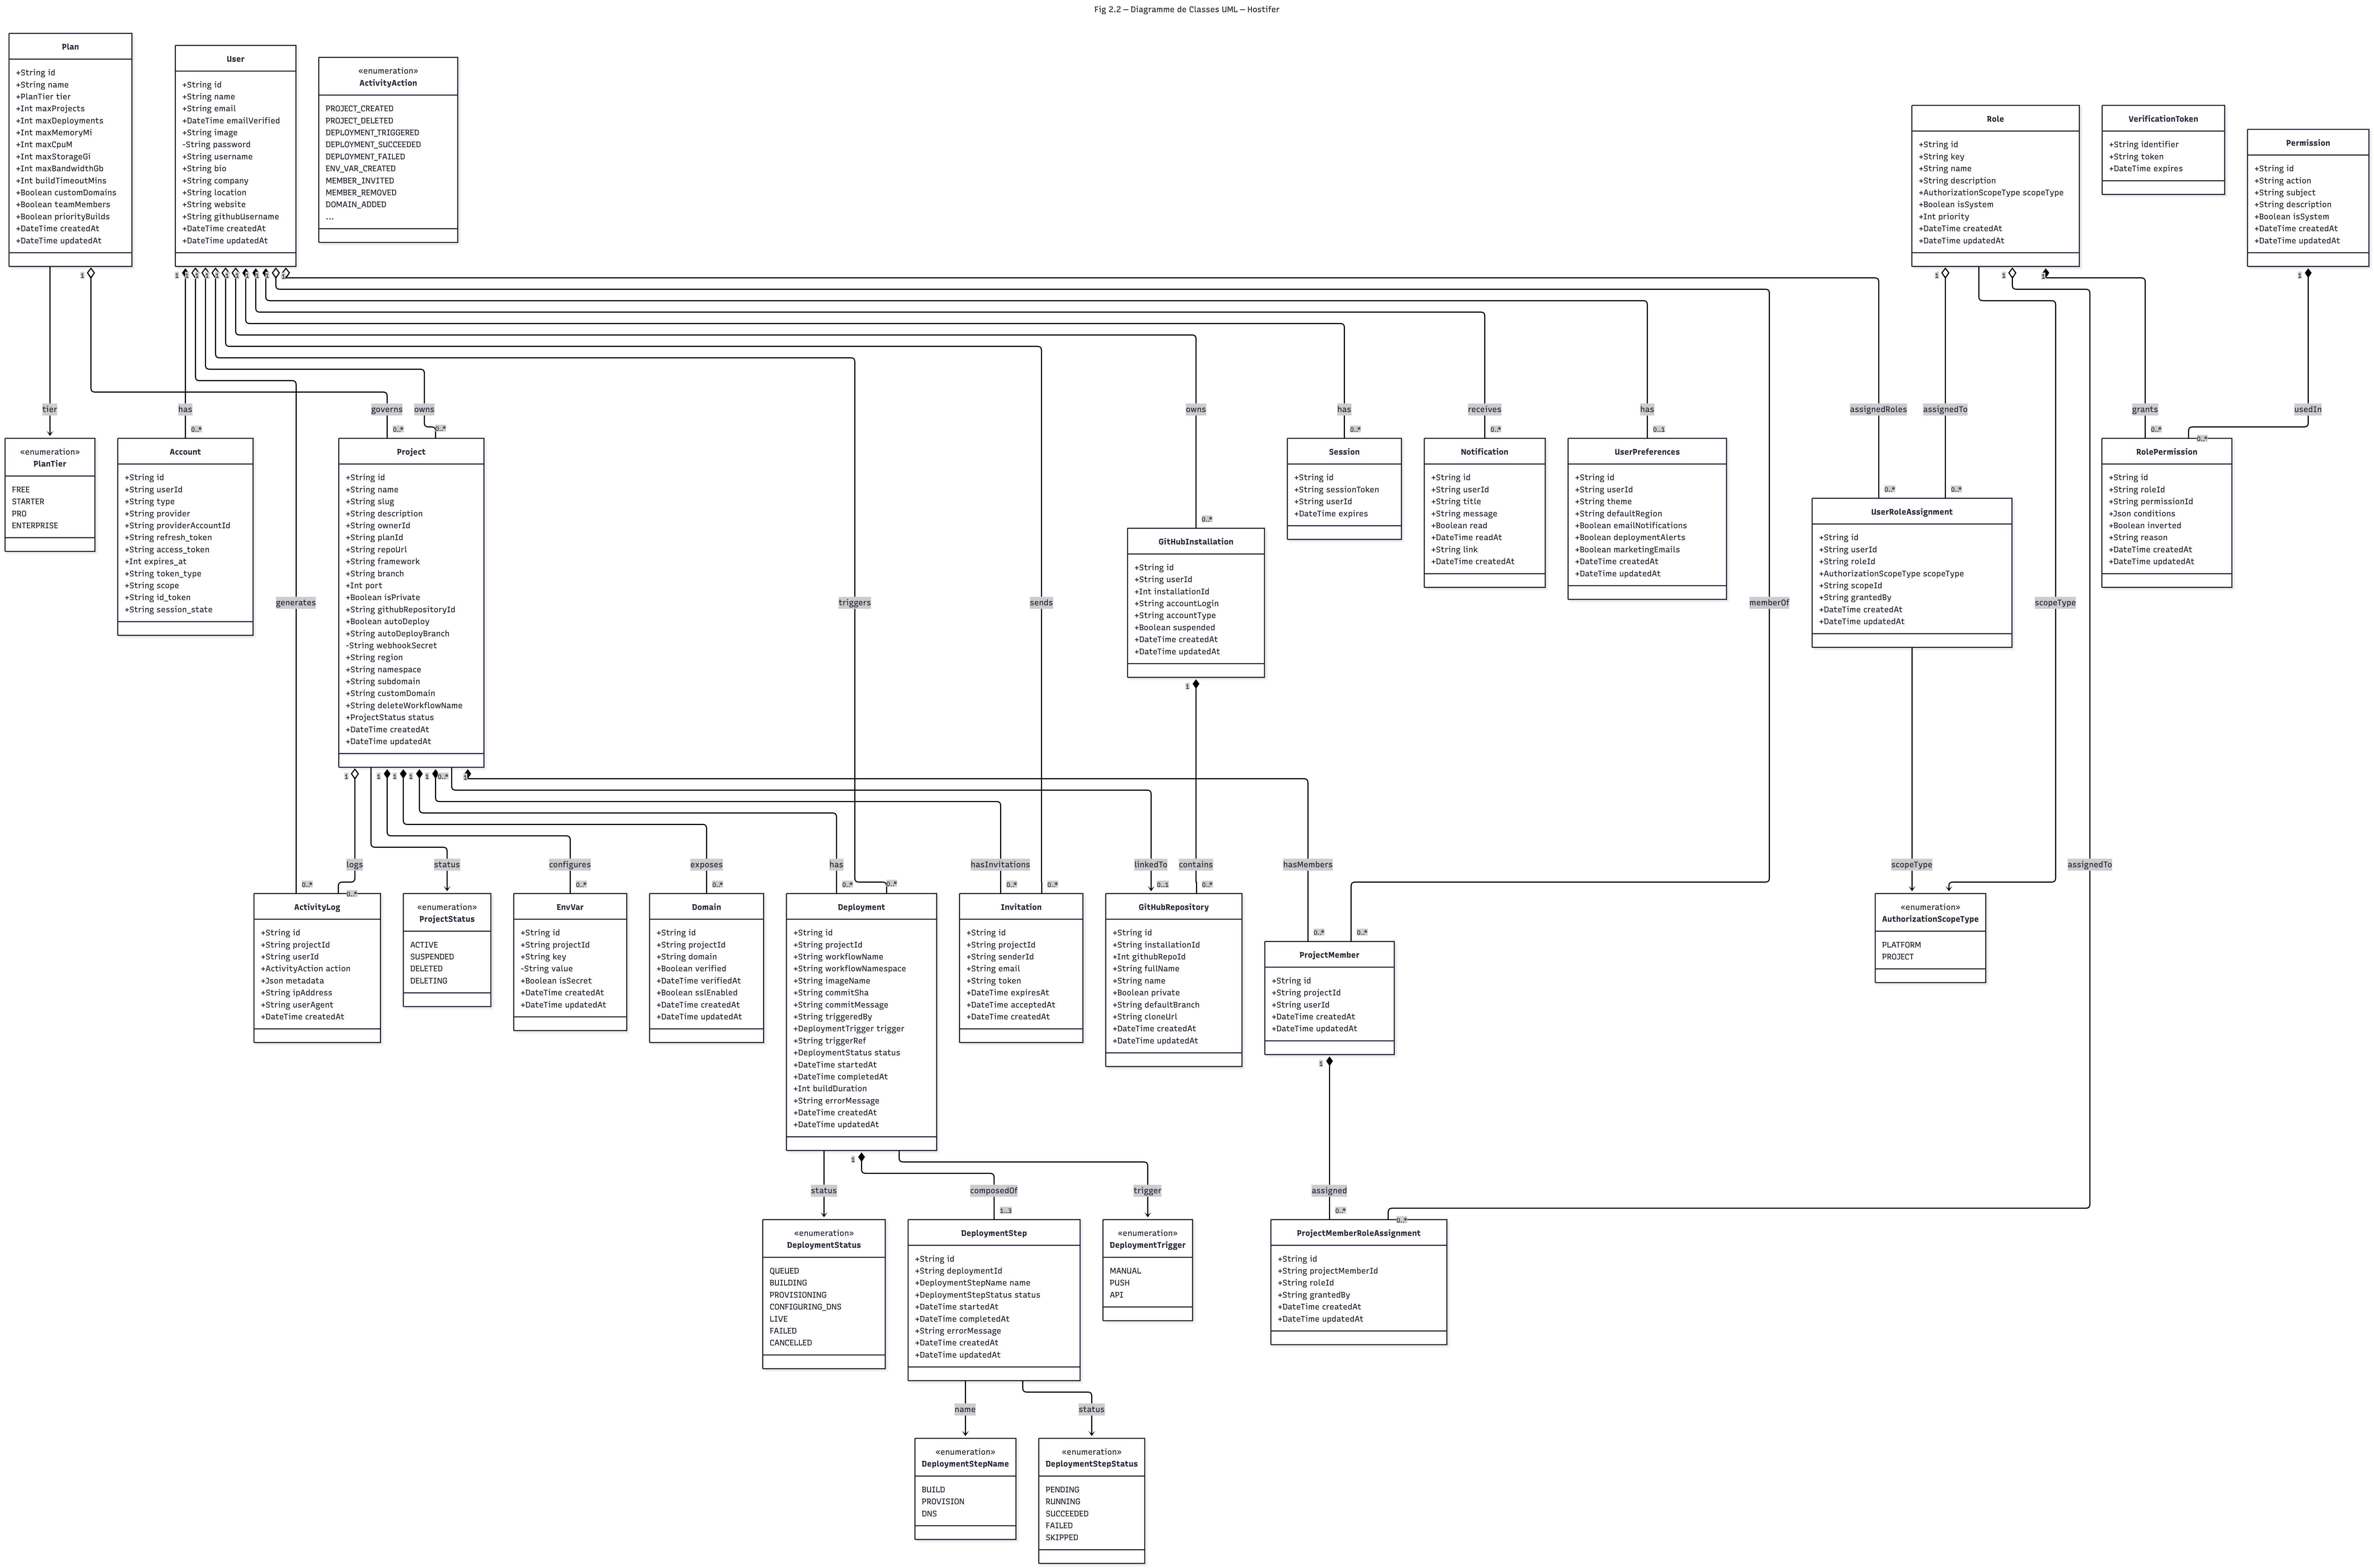
\includegraphics[width=1\linewidth]{5-Chapters/Chapter2/diagrams/class-diagram.png}
	\caption{Diagramme de classes UML complet (User, Project, Deployment, DeploymentStep, EnvVar, Plan, GitHubInstallation, GitHubRepository, ActivityLog, Notification, Domain)}
	\label{fig:2.2}
\end{figure}

\subsection{Modèle Entité-Association}

% Content here

\begin{figure}[h]
	\centering
	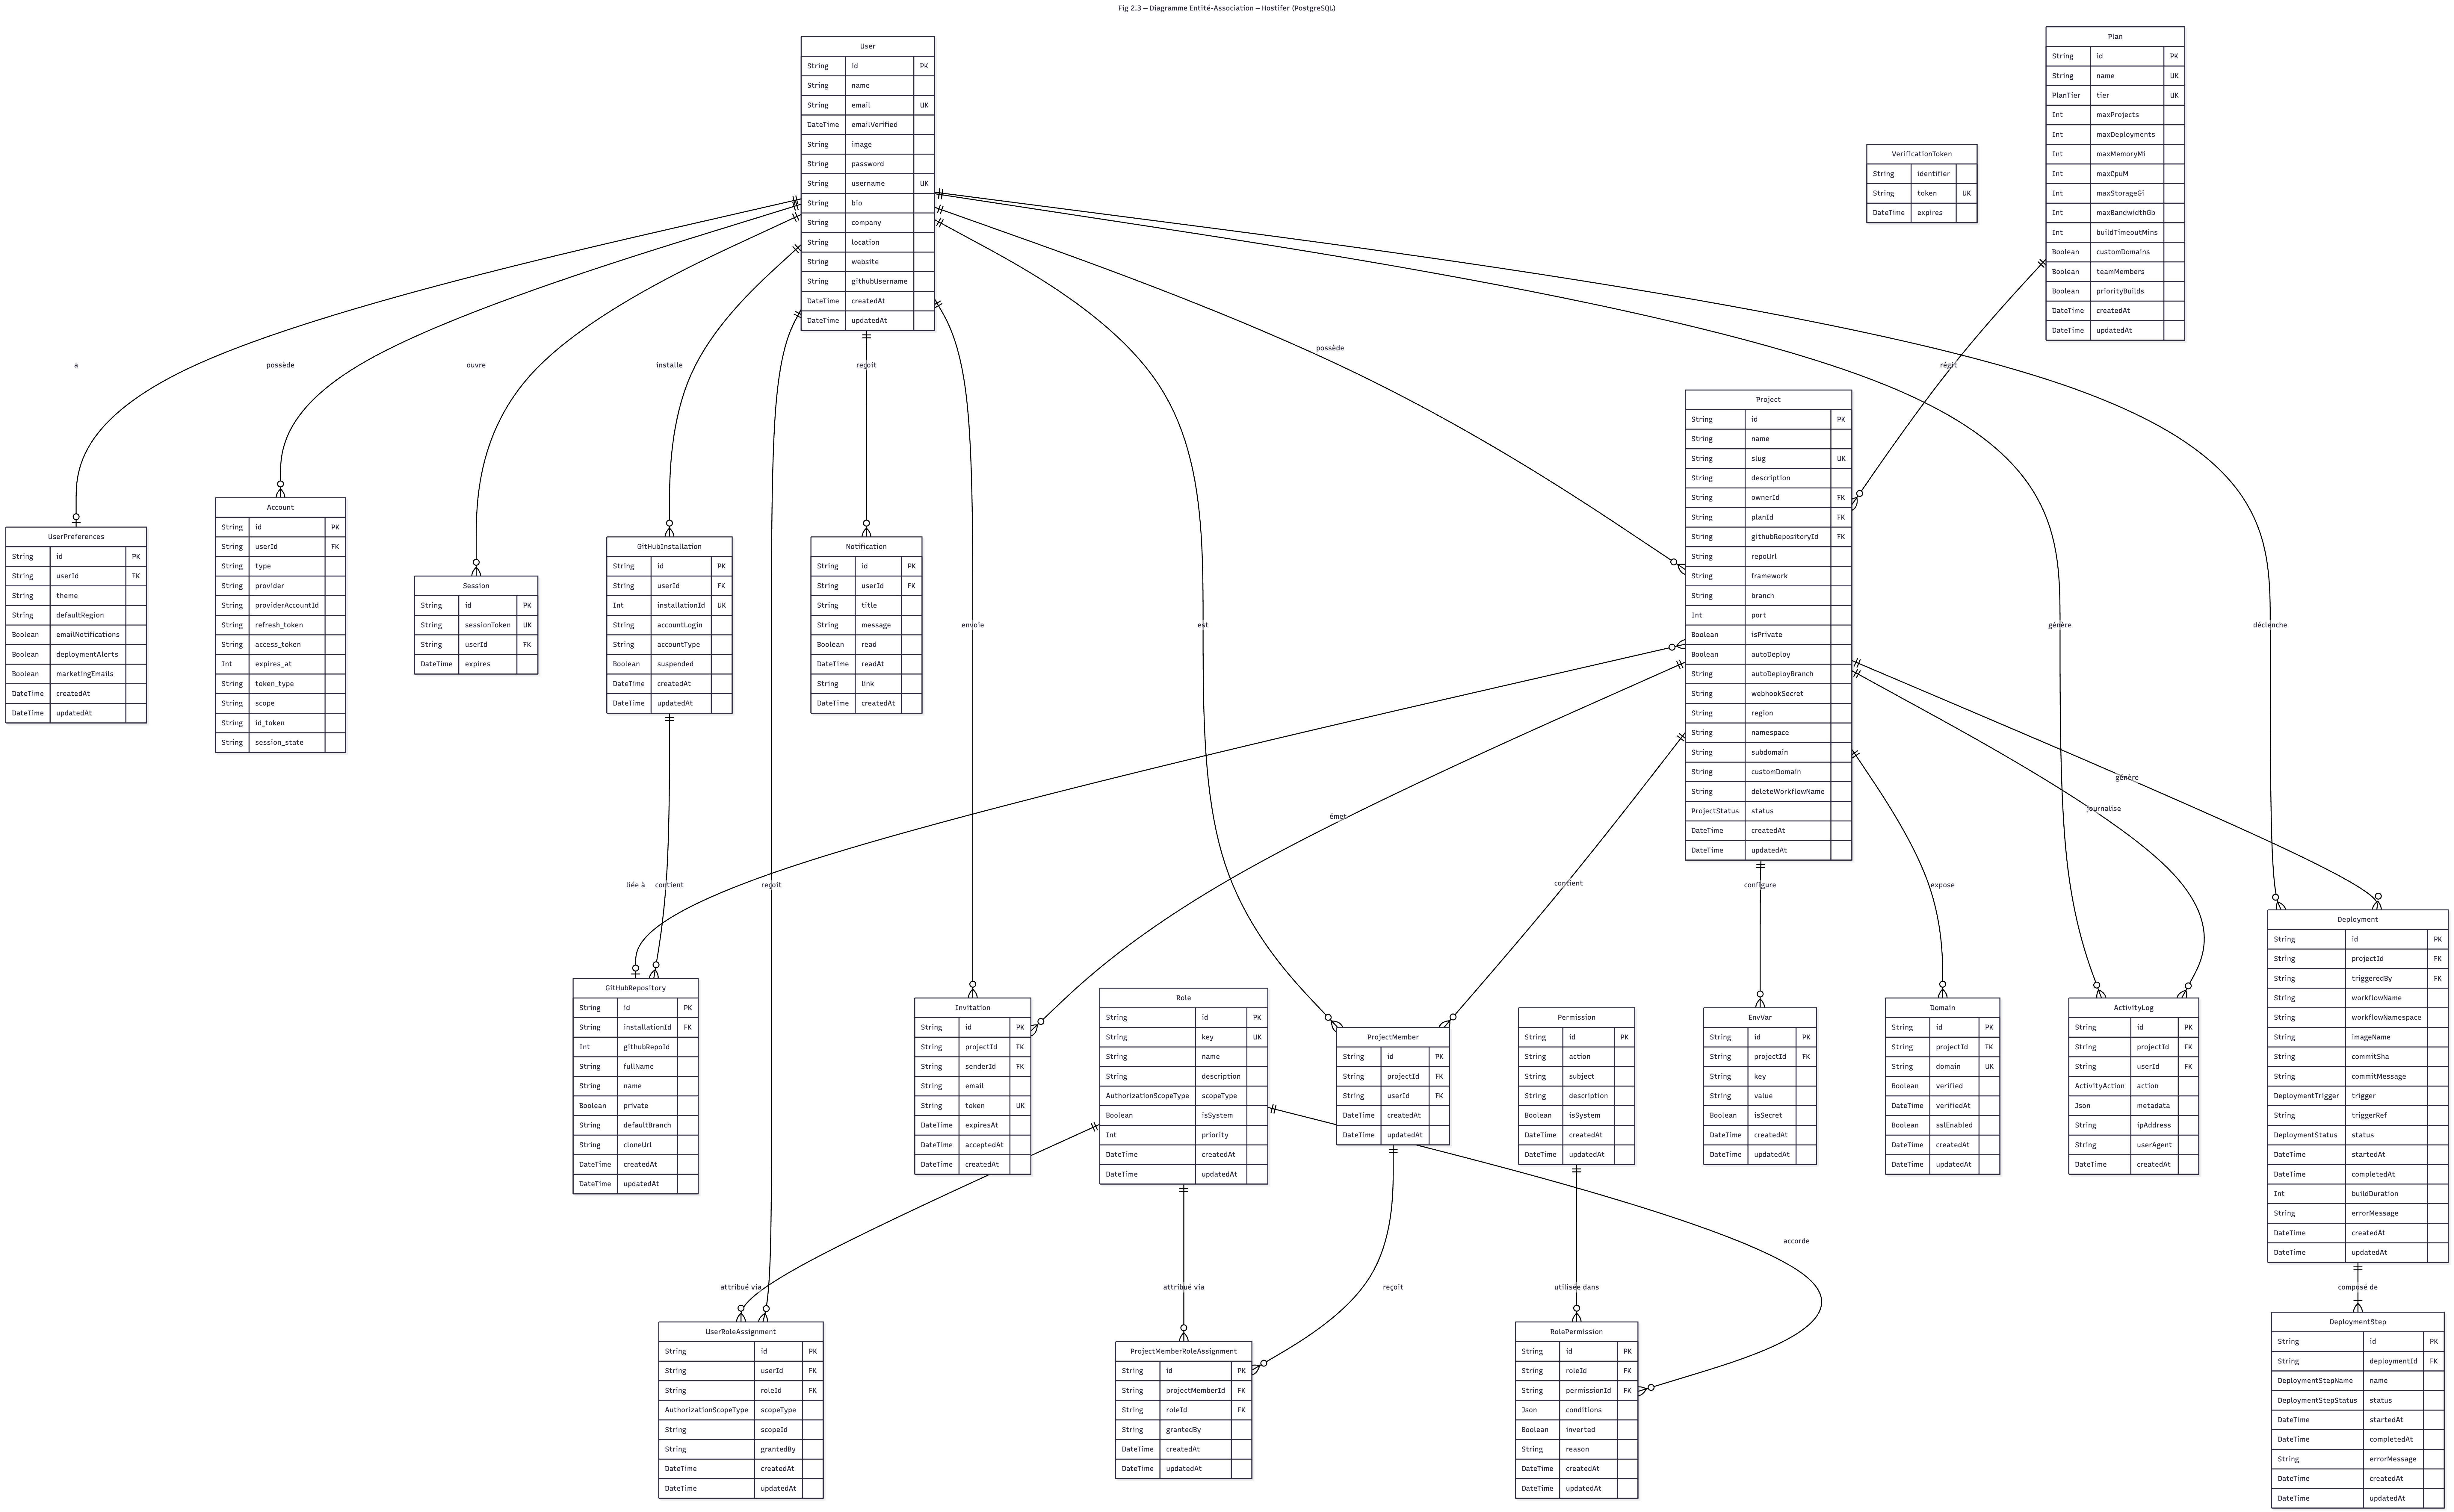
\includegraphics[width=1\linewidth]{5-Chapters/Chapter2/diagrams/Entite-relation.png}
	\caption{Diagramme Entité-Association de la base de données PostgreSQL avec cardinalités}
	\label{fig:2.3}
\end{figure}

% ------------------------------------------------------------
\subsection{Description des entités principales}
% ------------------------------------------------------------

La modélisation des entités constitue le socle de la couche de persistance de la plateforme. Chaque entité est implémentée sous forme de modèle Prisma ORM et correspond à une table dans la base de données PostgreSQL. Les tableaux suivants décrivent, pour chaque entité principale, l'ensemble des attributs avec leurs types de données, leurs contraintes d'intégrité, et leurs relations avec les autres entités du schéma.

% ── Tableau 2.4 — Entité User ───────────────────────────────
\begin{table}[htbp]
\caption{Description de l'entité \texttt{User}}
\label{tab:entity-user}
\centering
\renewcommand{\arraystretch}{1.3}
\begin{tabular}{|p{3cm}|p{2.5cm}|p{3.5cm}|p{4cm}|}
\hline
\textbf{Attribut} & \textbf{Type} & \textbf{Contraintes} & \textbf{Description} \\
\hline
\texttt{id} & \texttt{String} & PK, unique, \texttt{cuid()} & Identifiant unique de l'utilisateur généré automatiquement \\
\hline
\texttt{email} & \texttt{String} & unique, non null & Adresse email de l'utilisateur, utilisée pour l'authentification \\
\hline
\texttt{password} & \texttt{String?} & nullable & Mot de passe haché (bcrypt) ; null si authentification OAuth uniquement \\
\hline
\texttt{name} & \texttt{String?} & nullable & Nom complet de l'utilisateur \\
\hline
\texttt{avatarUrl} & \texttt{String?} & nullable & URL de l'avatar (fourni par GitHub OAuth) \\
\hline
\texttt{role} & \texttt{Enum} & non null, défaut \texttt{USER} & Rôle de l'utilisateur : \texttt{USER} ou \texttt{ADMIN} \\
\hline
\texttt{githubId} & \texttt{String?} & unique, nullable & Identifiant GitHub de l'utilisateur ; null si inscription email \\
\hline
\texttt{refreshToken} & \texttt{String?} & nullable & Dernier jeton de rafraîchissement JWT émis, haché en base \\
\hline
\texttt{createdAt} & \texttt{DateTime} & non null, défaut \texttt{now()} & Date et heure de création du compte \\
\hline
\texttt{updatedAt} & \texttt{DateTime} & non null, \texttt{@updatedAt} & Date et heure de la dernière mise à jour \\
\hline
\multicolumn{4}{|l|}{\textbf{Relations}} \\
\hline
\texttt{projects} & \texttt{Project[]} & — & Projets dont l'utilisateur est propriétaire \\
\hline
\texttt{memberships} & \texttt{ProjectMember[]} & — & Appartenances à des projets en tant que membre d'équipe \\
\hline
\texttt{installations} & \texttt{GitHubInstallation[]} & — & Installations GitHub OAuth associées au compte \\
\hline
\texttt{activityLogs} & \texttt{ActivityLog[]} & — & Journal des actions effectuées par l'utilisateur \\
\hline
\texttt{notifications} & \texttt{Notification[]} & — & Notifications reçues par l'utilisateur \\
\hline
\end{tabular}
\end{table}

% ── Tableau 2.5 — Entité Project ────────────────────────────
\begin{table}[htbp]
\caption{Description de l'entité \texttt{Project}}
\label{tab:entity-project}
\centering
\renewcommand{\arraystretch}{1.3}
\begin{tabular}{|p{3cm}|p{2.5cm}|p{3.5cm}|p{4cm}|}
\hline
\textbf{Attribut} & \textbf{Type} & \textbf{Contraintes} & \textbf{Description} \\
\hline
\texttt{id} & \texttt{String} & PK, unique, \texttt{cuid()} & Identifiant unique du projet \\
\hline
\texttt{name} & \texttt{String} & non null & Nom du projet, utilisé comme sous-domaine de l'URL publique \\
\hline
\texttt{slug} & \texttt{String} & unique, non null & Version normalisée du nom, utilisée dans les ressources Kubernetes et les URLs \\
\hline
\texttt{ownerId} & \texttt{String} & FK → \texttt{User.id}, non null & Référence à l'utilisateur propriétaire du projet \\
\hline
\texttt{repoUrl} & \texttt{String} & non null & URL du dépôt GitHub source \\
\hline
\texttt{repoName} & \texttt{String} & non null & Nom du dépôt GitHub (format \texttt{owner/repo}) \\
\hline
\texttt{branch} & \texttt{String} & non null, défaut \texttt{"main"} & Branche de déploiement par défaut \\
\hline
\texttt{framework} & \texttt{String?} & nullable & Framework détecté automatiquement lors du dernier build \\
\hline
\texttt{planId} & \texttt{String} & FK → \texttt{Plan.id}, non null & Plan tarifaire associé au projet (détermine les quotas de ressources) \\
\hline
\texttt{autoDeploy} & \texttt{Boolean} & non null, défaut \texttt{false} & Active le déploiement automatique sur événement \texttt{push} GitHub \\
\hline
\texttt{webhookSecret} & \texttt{String?} & nullable & Secret HMAC pour la validation des événements webhook GitHub \\
\hline
\texttt{installationId} & \texttt{String} & FK → \texttt{GitHubInstallation.id}, non null & Installation GitHub permettant l'accès au dépôt \\
\hline
\texttt{namespace} & \texttt{String?} & unique, nullable & Namespace Kubernetes alloué au projet lors du premier déploiement \\
\hline
\texttt{publicUrl} & \texttt{String?} & nullable & URL publique de l'application déployée \\
\hline
\texttt{createdAt} & \texttt{DateTime} & non null, défaut \texttt{now()} & Date et heure de création du projet \\
\hline
\texttt{updatedAt} & \texttt{DateTime} & non null, \texttt{@updatedAt} & Date et heure de la dernière mise à jour \\
\hline
\multicolumn{4}{|l|}{\textbf{Relations}} \\
\hline
\texttt{owner} & \texttt{User} & FK → \texttt{User} & Utilisateur propriétaire du projet \\
\hline
\texttt{plan} & \texttt{Plan} & FK → \texttt{Plan} & Plan tarifaire définissant les quotas de ressources \\
\hline
\texttt{deployments} & \texttt{Deployment[]} & — & Historique de tous les déploiements du projet \\
\hline
\texttt{envVars} & \texttt{EnvVar[]} & — & Variables d'environnement associées au projet \\
\hline
\texttt{members} & \texttt{ProjectMember[]} & — & Membres de l'équipe ayant accès au projet \\
\hline
\texttt{domains} & \texttt{Domain[]} & — & Domaines personnalisés associés au projet \\
\hline
\texttt{activityLogs} & \texttt{ActivityLog[]} & — & Journal des actions effectuées sur le projet \\
\hline
\end{tabular}
\end{table}

% ── Tableau 2.6 — Entité Deployment ─────────────────────────
\begin{table}[htbp]
\caption{Description de l'entité \texttt{Deployment}}
\label{tab:entity-deployment}
\centering
\renewcommand{\arraystretch}{1.3}
\begin{tabular}{|p{3cm}|p{2.5cm}|p{3.5cm}|p{4cm}|}
\hline
\textbf{Attribut} & \textbf{Type} & \textbf{Contraintes} & \textbf{Description} \\
\hline
\texttt{id} & \texttt{String} & PK, unique, \texttt{cuid()} & Identifiant unique du déploiement \\
\hline
\texttt{projectId} & \texttt{String} & FK → \texttt{Project.id}, non null & Référence au projet auquel appartient ce déploiement \\
\hline
\texttt{status} & \texttt{Enum} & non null, défaut \texttt{QUEUED} & État courant du déploiement (voir cycle de vie ci-dessous) \\
\hline
\texttt{commitSha} & \texttt{String?} & nullable & Hash du commit Git déployé \\
\hline
\texttt{commitMessage} & \texttt{String?} & nullable & Message du commit Git associé au déploiement \\
\hline
\texttt{branch} & \texttt{String} & non null & Branche Git source du déploiement \\
\hline
\texttt{imageTag} & \texttt{String?} & nullable & Tag de l'image OCI construite et poussée vers le registre interne \\
\hline
\texttt{argoWorkflowName} & \texttt{String?} & nullable & Nom du workflow Argo Workflows soumis pour ce déploiement \\
\hline
\texttt{buildDuration} & \texttt{Int?} & nullable & Durée de l'étape Build en secondes \\
\hline
\texttt{totalDuration} & \texttt{Int?} & nullable & Durée totale du déploiement (Build + Provision + DNS) en secondes \\
\hline
\texttt{triggeredBy} & \texttt{Enum} & non null & Origine du déclenchement : \texttt{MANUAL} ou \texttt{WEBHOOK} \\
\hline
\texttt{createdAt} & \texttt{DateTime} & non null, défaut \texttt{now()} & Date et heure de création de l'entrée de déploiement \\
\hline
\texttt{updatedAt} & \texttt{DateTime} & non null, \texttt{@updatedAt} & Date et heure de la dernière mise à jour de l'état \\
\hline
\texttt{finishedAt} & \texttt{DateTime?} & nullable & Date et heure de fin du déploiement (succès ou échec) \\
\hline
\multicolumn{4}{|l|}{\textbf{Relations}} \\
\hline
\texttt{project} & \texttt{Project} & FK → \texttt{Project} & Projet parent du déploiement \\
\hline
\texttt{steps} & \texttt{DeploymentStep[]} & — & Étapes détaillées du pipeline (Build, Provision, DNS) \\
\hline
\multicolumn{4}{|l|}{\textbf{Valeurs de l'énumération \texttt{DeploymentStatus}}} \\
\hline
\multicolumn{4}{|p{13cm}|}{\parbox[t]{13cm}{
\raggedright
\texttt{QUEUED} → \texttt{BUILDING} → \texttt{PROVISIONING} → \texttt{CONFIGURING\_DNS} → \texttt{LIVE}\par
Transitions d'échec possibles depuis tout état actif : → \texttt{FAILED}\par
Annulation possible depuis tout état actif : → \texttt{CANCELLED}
}} \\
\hline
\end{tabular}
\end{table}

% Content here

\begin{table}[h]
	\centering
	\caption{Description de l'entité User (attributs, types, contraintes)}
	\label{tab:2.4}
\end{table}

\begin{table}[h]
	\centering
	\caption{Description de l'entité Project}
	\label{tab:2.5}
\end{table}

\begin{table}[h]
	\centering
	\caption{Description de l'entité Deployment}
	\label{tab:2.6}
\end{table}

\section{Modélisation comportementale}

\subsection{Diagrammes de séquence}

% Content here

\begin{figure}[h]
	\centering
	\fcolorbox{black}{black}{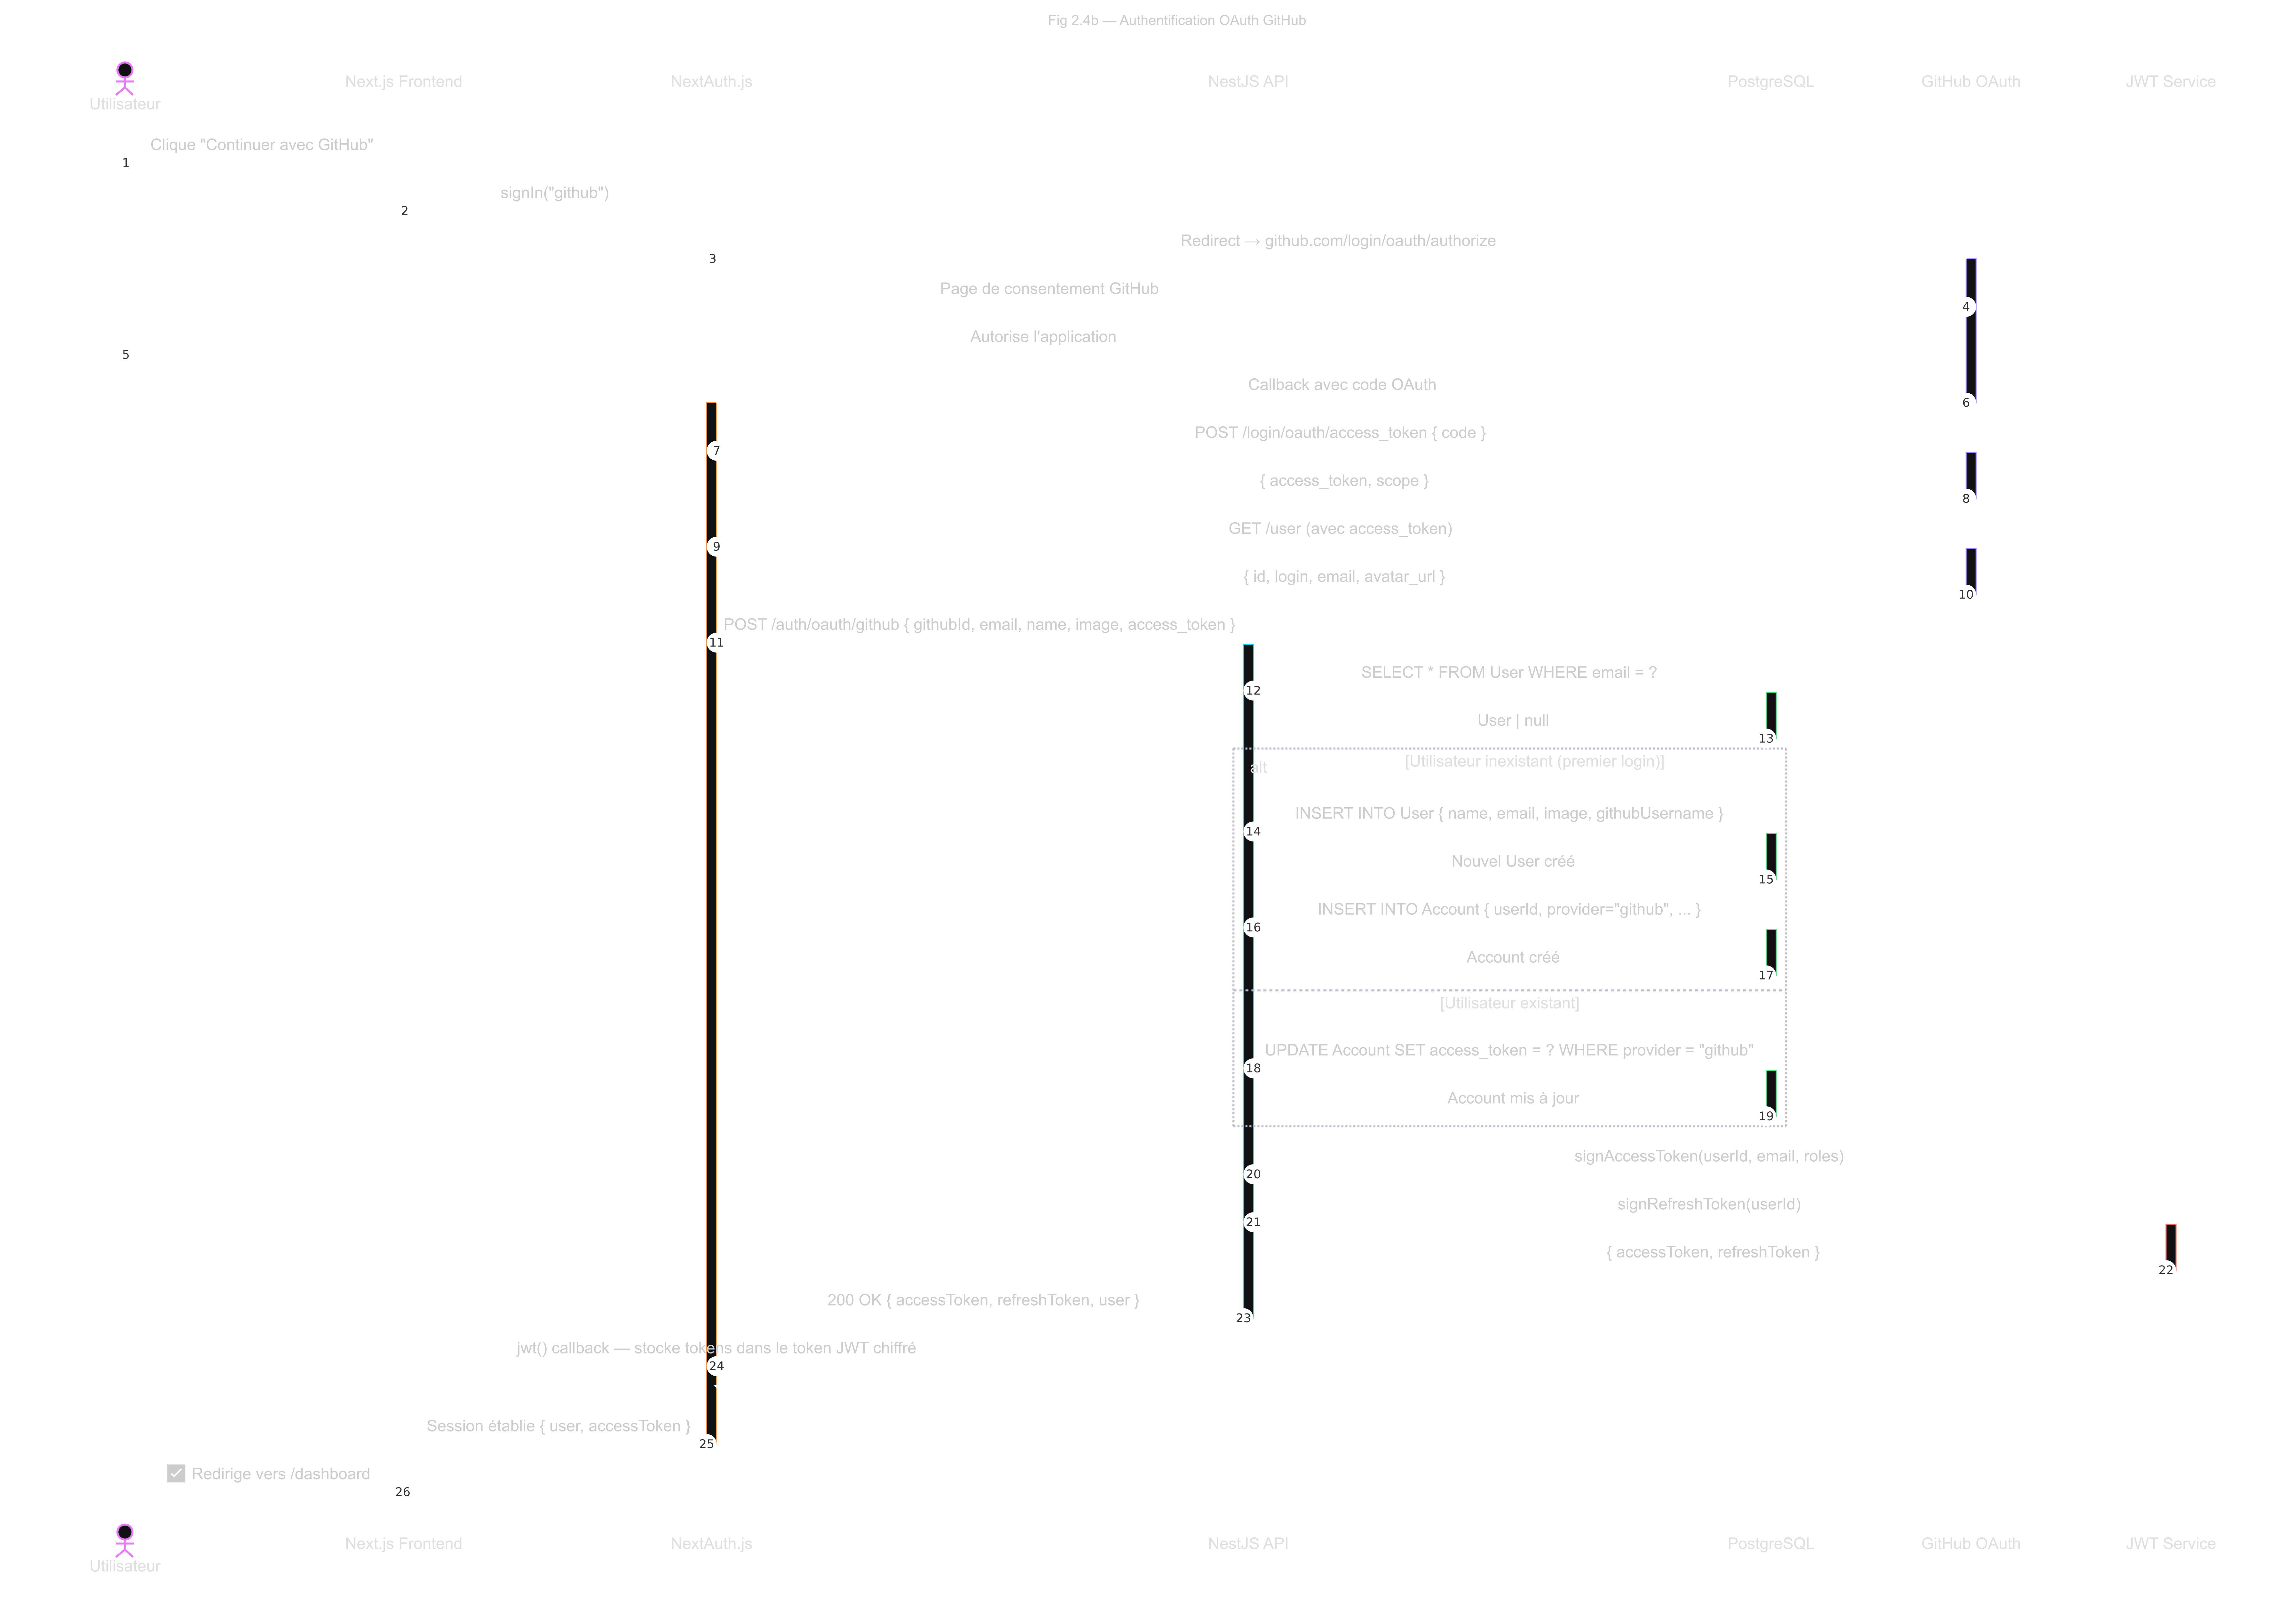
\includegraphics[width=1\linewidth]{5-Chapters/Chapter2/diagrams/github_oauth.png}}
	\caption{Diagramme de séquence : Authentification (NextJS → NestJS → PostgreSQL → JWT)}
	\label{fig:2.4}
\end{figure}

\begin{figure}[h]
	\centering
	\caption{Diagramme de séquence : Déclenchement d'un déploiement (Frontend → NestJS → Argo Workflows → Build Job → Registry → Helm → DNS)}
	\label{fig:2.5}
\end{figure}

\begin{figure}[h]
	\centering
	\caption{Diagramme de séquence : Streaming des logs en temps réel (Builder Pod → Promtail → Loki → NestJS SSE → Browser)}
	\label{fig:2.6}
\end{figure}

\begin{figure}[h]
	\centering
	\caption{Diagramme de séquence : Webhook CI/CD GitHub Push (GitHub → NestJS → DeploymentsService → Argo Workflows)}
	\label{fig:2.7}
\end{figure}

\subsection{Diagrammes d'activité}

% Content here

\begin{figure}[h]
	\centering
	\caption{Diagramme d'activité du pipeline de déploiement complet (Build → Provision → DNS → Live)}
	\label{fig:2.8}
\end{figure}

\begin{figure}[h]
	\centering
	\caption{Diagramme d'activité de la détection de framework et génération du plan Railpack}
	\label{fig:2.9}
\end{figure}

\subsection{Diagramme d'états}

% Content here

\begin{figure}[h]
	\centering
	\caption{Diagramme d'états d'un Deployment (QUEUED → BUILDING → PROVISIONING → CONFIGURING\_DNS → LIVE / FAILED / CANCELLED)}
	\label{fig:2.10}
\end{figure}

\section{Architecture technique globale}

\subsection{Vue d'ensemble de l'architecture}

% Content here

\begin{figure}[h]
	\centering
	\caption{Schéma d'architecture générale de Hostifer : couche client (NextJS), couche API (NestJS), couche orchestration (Argo Workflows), couche infrastructure (Kubernetes, Buildkit, Registry, Loki, Vault), couche réseau (Traefik, Cloudflare, cert-manager)}
	\label{fig:2.11}
\end{figure}

\subsection{Architecture multi-tenant}

% Content here

\begin{figure}[h]
	\centering
	\caption{Schéma d'isolation multi-tenant : Namespace par projet, NetworkPolicy bloquant le trafic inter-tenant, ressources quotas par plan}
	\label{fig:2.12}
\end{figure}

\begin{table}[h]
	\centering
	\caption{Ressources allouées par profil d'allocation (CPU request/limit, RAM request/limit, stockage, pods max). Les métriques d'autoscaling supportées et les comportements HPA/VPA autorisés par profil sont indiqués dans la grille}
	\label{tab:2.7}
\end{table}

\subsection{Architecture du pipeline de build}

% Content here

\begin{figure}[h]
	\centering
	\caption{Schéma du pipeline de build (Job Kubernetes Go binary → Railpack CLI → Buildkitd Deployment → Registry interne)}
	\label{fig:2.13}
\end{figure}

\subsection{Architecture de collecte des logs}

% Content here

\begin{figure}[h]
	\centering
	\caption{Schéma de la chaîne de collecte et streaming des logs (Pod stdout → Promtail DaemonSet → Loki → SSE → Browser)}
	\label{fig:2.14}
\end{figure}

\subsection{Architecture de gestion des secrets}

% Content here

\begin{figure}[h]
	\centering
	\caption{Schéma de gestion des secrets avec HashiCorp Vault et External Secrets Operator}
	\label{fig:2.15}
\end{figure}

\section{Choix technologiques}

\subsection{Justification des technologies retenues}

% Content here

\begin{table}[h]
	\centering
	\caption{Tableau des choix technologiques (composant, technologie retenue, alternatives considérées, justification du choix)}
	\label{tab:2.8}
\end{table}